\documentclass{report}
\usepackage{setspace}
\usepackage{caption}

\pagestyle{plain}
\usepackage[table]{xcolor}
\usepackage{color}
\usepackage{amssymb,graphicx,color}
\usepackage{subcaption}
\usepackage{amsfonts}
\usepackage{latexsym}
% \usepackage{a4wide}
\usepackage{amsmath}
\usepackage{multirow}
\usepackage{makecell}
\usepackage{xcolor}
\usepackage{mathtools}
\usepackage{float}

\allowdisplaybreaks

\newcommand\todo[1]{\textcolor{red}{#1}}
\DeclareMathOperator*{\argmax}{arg\,max}
\DeclareMathOperator*{\argmin}{arg\,min}

\graphicspath{ {/home/stensootla/projects/adversarial-on-disentangled/text/figures/} }

\newtheorem{theorem}{THEOREM}
\newtheorem{lemma}[theorem]{LEMMA}
\newtheorem{corollary}[theorem]{COROLLARY}
\newtheorem{proposition}[theorem]{PROPOSITION}
\newtheorem{remark}[theorem]{REMARK}
\newtheorem{definition}[theorem]{DEFINITION}
\newtheorem{fact}[theorem]{FACT}

\newtheorem{problem}[theorem]{PROBLEM}
\newtheorem{exercise}[theorem]{EXERCISE}
\def \set#1{\{#1\} }

\newenvironment{proof}{
PROOF:
\begin{quotation}}{
$\Box$ \end{quotation}}

\newcommand{\nats}{\mbox{\( \mathbb N \)}}
\newcommand{\rat}{\mbox{\(\mathbb Q\)}}
\newcommand{\rats}{\mbox{\(\mathbb Q\)}}
\newcommand{\reals}{\mbox{\(\mathbb R\)}}
\newcommand{\ints}{\mbox{\(\mathbb Z\)}}

\definecolor{light-gray}{gray}{0.90}

%%%%%%%%%%%%%%%%%%%%%%%%%%


\title{{ 
\includegraphics[scale=.5,natwidth=294,natheight=84]{ucl_logo}}\\
{{\Huge Investigating the Robustness of Disentangled Variational Autoencoders to Adversarial Examples}}\\}
\date{Submission date: 10.08.2018}
\author{Sten Sootla\thanks{
{\bf Disclaimer:}
This report is submitted as part requirement for the MSc degree in Computational Statistics and Machine Learning at UCL. It is substantially the result of my own work except where explicitly indicated in the text. The report may be freely copied and distributed provided the source is explicitly acknowledged.}
\\ \\
Computational Statistics and Machine Learning\\ \\
Supervised by Dr. Cristina Calnegru and Dr. John Shawe-Taylor
}


\begin{document}
 
\onehalfspacing
\maketitle
\begin{abstract}
Summarise your report concisely.
\end{abstract}
\tableofcontents
\setcounter{page}{1}


\chapter{Introduction}


% 1. Adversarial examples

\noindent In recent years, deep neural networks have shown impressive results in various supervised pattern recognition tasks, including image classification \cite{alexnet, resnet}, object detection \cite{rcnn}, and machine translation \cite{nmt}. Capitalizing on the resurgence of deep neural models in the supervised learning domain, unsupervised methods have also gone through a renaissance, as they have moved from modelling relatively simple datasets \cite{rbm, helmholtz} to being able to capture exceedingly complex real-world distributions \cite{began, musicvae}. One of the most prominent generative models behind these successes is the variational autoencoder (VAE) \cite{vae}, which merges conventional probabilistic methods with deep learning, using neural networks to parameterize both the generative and approximate posterior distributions in the the evidence lower bound. \\

\noindent The successes of these "neural" models, consisting mainly of stacks of layers, each of which is composed of a linear mapping followed by a nonlinearity, can be attributed to the fact that they can theoretically approximate arbitarily complex functions \cite{Cybenko1989}. However, as the appropriate functions are discovered automatically via a black-box optimization algorithm (e.g. gradient descent or an evolutionary method), the models can have counter-inuitive properties \cite{intriguing-properties}. \\

\noindent First, the resulting decision boundaries of the trained networks are often non-interpretable and unintuitive. Indeed, one of the most well-known and intriguing failure modes of most machine learning algorithms is the existence of adversarial examples - datapoints that are perceptually very close to examples from the original training distribution, but which fool the model with high confidence \cite{intriguing-properties}. The fact that state-of-the-art deep learning models are subject to such adversarial perturbations challenges the narrative that they are unreasonably effective in generalizing outside the distribution they are trained on \cite{bengio-deep-architectures}. More practically, as the models under discussion are being pushed into production for use in semi-autonomous vehicles \cite{nvidia-self-driving-cars}, drones \cite{drones}, surveillance cameras \cite{surveillance-cameras} and malware detection pipelines \cite{malware}, the existence of adversarial examples poses a security threat with possible real-world consequences. \\

\noindent Second, the internal representations learnt by deep neural networks are infamously complex and hard to analyse. Indeed, Szegedy et. al. \cite{intriguing-properties} have shown that directions along the coordinate axes are often no more semantically meaningful than other directions in the latent space. Similarly, Morcos et. al. \cite{importance-single-directions} discovered that even if there exist individual units that are interpretable, they are no more important to the task at hand than neurons that don't exhibit clear correlation with specific semantic concepts. In other words, the models learn representations where units are \textit{entangled} - each individual semnatically meaningful factor of variation in the input is explained by a combination of hidden units, as opposed to a single neuron. \\

\noindent It has been argued \cite{bengio-representation} that such entangled representations are suboptimal for generalization, and incorporating inductive biases which would steer the representations towards \textit{disentanglement} would be beneficial. Indeed, it seems intuitively plausible that generalizing to novel configurations of concepts that were not encountered in the training distribution is easiest when relevant factors of variation in the input data are aligned with individual neurons in the latent space. Validating the intuition, such representations have recently shown promising results in zero-shot transfer learning \cite{darla}, semi-supervised learning \cite{dgpose}, and life-long learning \cite{vase}. \\

\noindent This thesis investigates the possible relationship between the two intriguing properties of neural networks outlined above: the counter-intuitive decision boundaries on one hand, and the apparent overly complex internal representations on the other. It is reasonable to assume the existence of such a connection, since one way to construct adversarial examples for encoder-decoder type models is to perturb the source image in such a way that its internal representation would be close to the representation of some target image, while simultaneously meddling with the pixels of the source image as little as possible \cite{kos-gen-adv, tabacof-gen-adv}. The success of this methodology implies that variational autoencoders do not preserve the locality of inputs in their latent space. It has been argued, however, that models whose internal representation is disentangled encode nearby points in pixel space to similar representations in latent space as well \cite{beta-vae}. If true, we would expect such models to be significantly more robust to adversarial examples of this type. \\

\noindent To test the preceding hypothesis, we empirically evaluated the robustness of state-of-the-art disentanglement-inducing VAEs to adversarial examples \footnote{In the context of generative models, an adversarial example is a datapoint which is very similar to the original, untampered image, but whose reconstruction differs markedly from the original's. As an example, an adversarial image could look like a regular depiction of the digit two, but which is reconstructed as the digit four by the generative model.}, and compared the results to regular, entangled VAEs. The analyses were carried out for the MNIST handwritten images dataset \cite{mnist}. Surprisingly, it was found that disentangled generative models are actually \textit{less} robust to attacks on this dataset, contradicting our initial rationale. This stands in stark contrast to previous work by Alemi et. al. \cite{deep-variational-bottleneck}, which performed similar analysis for supervised models, but arrived at the opposite conclusion, highlighting a fundamental difference between generative and discriminative models when it comes to adversarial examples. \\

\noindent The thesis is organized as follows. In Chapter 2, a sufficiently in-depth overview of variational autoencoders, disentanglement, and adversarial examples is given. Chapter 3 outlines the experimental methodology, and provides exact details of the analyses done in this thesis for reproducibility. Chapter 4 gives the results of the experiments. 

\chapter{Related work and background}

This chapter introduces the preliminary topics that are integral to understanding the methods and results of this thesis, with the assumption that the reader is comfortable with the basics of discriminative methods in machine learning. In addition, it provides an overview of the most important previous works that are closely related to ours. \\

\noindent To fully appreciate deep generative models and the problems they are best suited to tackle, it is paramount to first be aware of the context that they operate in. To that end, a brief introduction to the probabilistic view of pattern recognition is given in the first section. The second section builds on the first, introducing the variational autoencoder. The third section focusses on how to regularize generative models such that the learnt representations would be disentangled. The last section introduces the general problem of adversarial examples, and discusses their applicability to generative models.

\section{Probabilistic learning and inference}

\subsection{Discriminative approach}

\noindent Usually, in the case of conventional supervised learning, one is concerned about capturing the probability distribution of some predefined labels, conditioned on a set of inputs. For example, in classification, we try to model the categorical distribution of possible classes, given an image (or some set of higher-level features derived from raw pixels) belonging to one of the categories. Relatedly, we could be interested in continuous conditional distributions, as one might be when trying to estimate the future earnings of a company based on its current key performance indicators. \\

\noindent As a concrete example, due to Bishop \cite{bishop-prml}, of how viewing machine learning through a probabilistc lens can yield useful insights into well-known methodologies, let us see how the ubiquitous sum-of-squares error function comes about naturally from a principled probabilistic approach. Suppose we have $N$ possibly high-dimensional training inputs $\mathbf{\boldsymbol{X}} = \{\boldsymbol{x}^{(1)}, \boldsymbol{x}^{(2)}, \dots, \boldsymbol{x}^{(n)}\}$, and their corresponding one-dimensional target values $\mathbf{t} = \{t^{(1)}, t^{(2)}, \dots, t^{(n)}\}$. Our uncertainty about the targets can be modelled as a Gaussian with a fixed precision $\beta$, whose mean is represented by a parameterized function $y(x; \boldsymbol{\theta})$ (e.g. an artificial neural network):

\[ p(t^{(i)}|\boldsymbol{x}^{(i)}; \boldsymbol{\theta}, \beta)  = \mathcal{N} (t^{(i)} | y(\boldsymbol{x}^{(i)}; \boldsymbol{\theta}), \beta^{-1}). \]

\bigskip

\noindent If we further assume that the given targets were drawn independently from this normal distribution, we can estimate the unknown parameters $\boldsymbol{\theta}$ and $\beta$ by maximizing the log-likelihood of the targets:
\begin{gather*}
\argmax_{\boldsymbol{\theta}} \log p(\mathbf{t}; \boldsymbol{\theta}) = \\
\argmax_{\boldsymbol{\theta}} \log \prod_{n=1}^N \mathcal{N}(t^{(n)} | y(\boldsymbol{x}^{(n)}; \boldsymbol{\theta}), \beta^{-1}) = \\
\argmax_{\boldsymbol{\theta}} \sum_{n=1}^N \log \mathcal{N}(t^{(n)} | y(\boldsymbol{x}^{(n)}; \boldsymbol{\theta}), \beta^{-1}) = \\
\argmax_{\boldsymbol{\theta}} \sum_{n=1}^N \log \Big(\frac{\beta}{2 \pi}\Big)^{\frac{1}{2}} e^{-\frac{\beta}{2} (t^{(n)} - y(\boldsymbol{x}^{(n)}; \boldsymbol{\theta}))^2} = \\
\argmax_{\boldsymbol{\theta}} \sum_{n=1}^N \frac{1}{2} (\log \beta - \log 2 \pi) {-\frac{\beta}{2} (t^{(n)} - y(\boldsymbol{x}^{(n)}; \boldsymbol{\theta}))^2} = \\
\argmin_{\boldsymbol{\theta}} \sum_{n=1}^N (t^{(n)} - y(\boldsymbol{x}^{(n)}; \boldsymbol{\theta}))^2,
\end{gather*} 

\noindent where the last equality follows from the fact that the first term inside the summation does not depend on the parameter $\boldsymbol{\theta}$, and that scaling the parameter-dependent term by a negative constant is equivalent to dropping the constant and turning the maximization problem into a minimization. With that, we have convinced ourselves that even in the usual discriminative setting, we are in fact making implicit use of a probabilistic approach to machine learning. \\

\subsection{Generative approach}

\noindent So far we have dealt with modelling the conditional distribution of the targets, given the inputs. Sometimes, however, we might be after the marginal distribution of the input data itself. Having such an object in hand, we are able to determine if an observed example has an unusually low probability of occurrence for anomaly detection \cite{vae-anomaly}, fill out missing dimensions of incomplete datapoints \cite{missing-data}, or sample new, realistic datapoints from the learnt density function \cite{vaegan}.  \\

\noindent Capturing the marginal distribution of the inputs is often somewhat more involved than it was in the conditional case discussed previously. This is largely due the fact that high-dimensional, multi-modal datapoints have complex densities whose modelling with well-known distributions would yield suboptimal results. In such situations, additional structure is often incorporated into the probabilistic models in the form of lower-dimensional latent variables. \\

\noindent The inclusion of such auxiliary variables is often motivated by the hierarchical nature of physical processes. For example, by thinking about how images could be constructed from a generative point of view, we might imagine that first it is decided which objects to lay onto the scene. Second, one might go into more detail and think about what individual parts do the objects consist of. Finally, the orientations of the edges might be decided upon, after which the actual imagine could be drawn out onto the canvas. Interestingly, having imposed such hierarchical dependecy structure on our model, we can also traverse the dependency graph bottom-up, reducing our uncertainty about the latents, given an observed datapoint. This inversion of the generative process is called inference, and plays a central role in this thesis. Figure \ref{fig:latent-vars} illustrates the generative and inferential processes just described. \\

\begin{figure}
\begin{center}
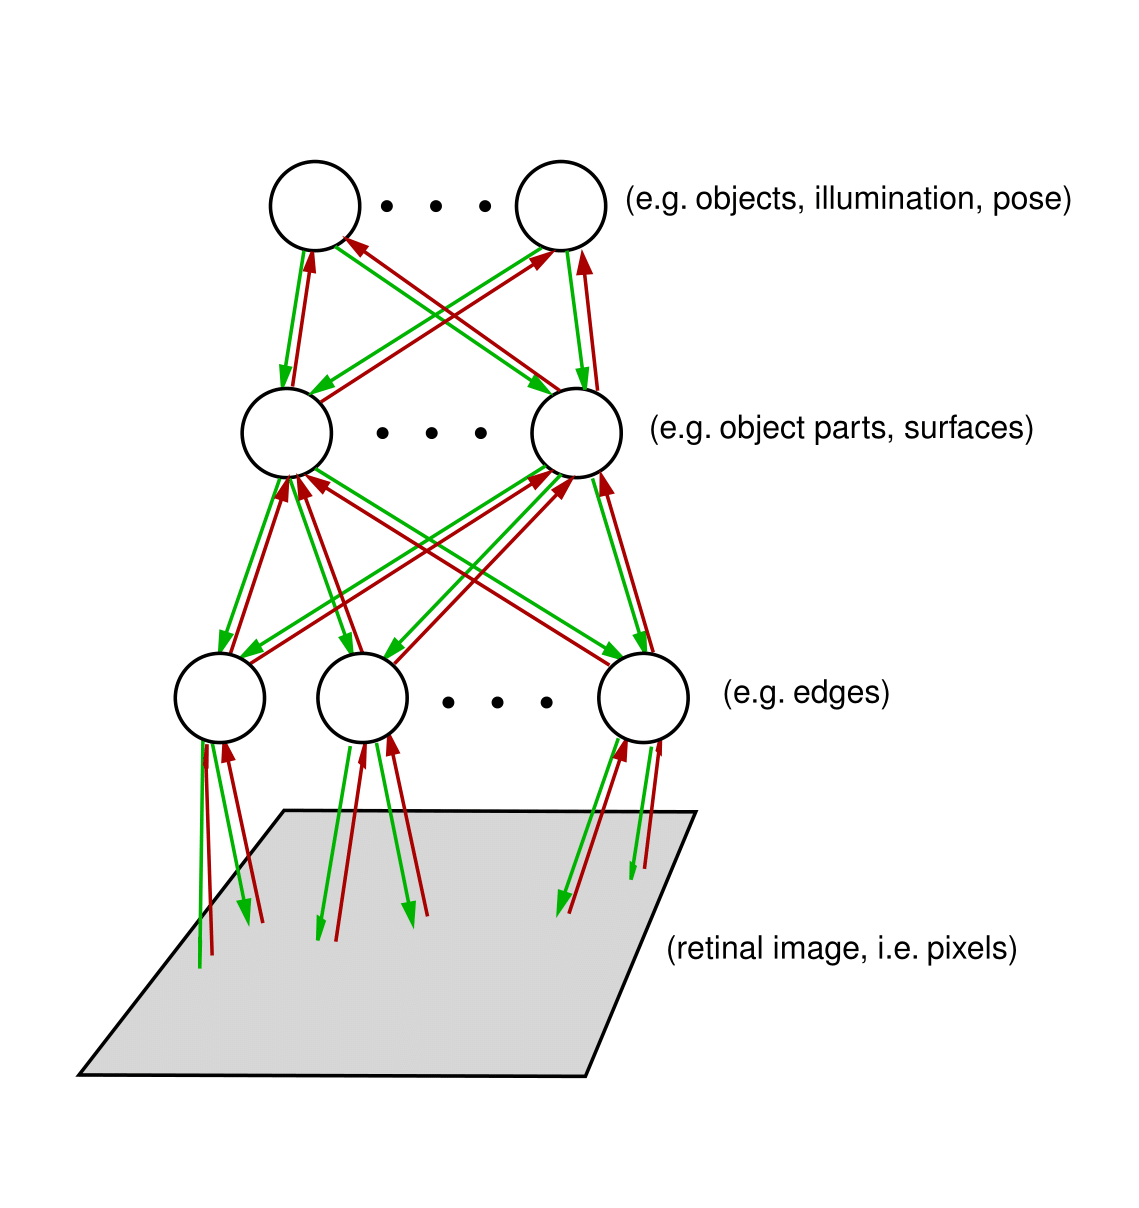
\includegraphics[width=0.5\textwidth,natwidth=1139,natheight=1208]{latentvar}
\caption{Illustration of a probabilistic model with latent variables. Green arrows represent the generative process, in which higher-level concepts guide the development of lower-level ones, eventually leading to the generation of each pixel in an image. Red arrows depict inference, in which case the goal it to infer the underlying causes of an obtained input. Reprinted from M. Sahani, 2018 \cite{gatsby-slide}.}
\label{fig:latent-vars}
\end{center}
\end{figure}

\noindent One immediate drawback to using more complicated latent variable models is that evaluating the likelihood turns out to be intractable, as one has to formally consider the probability of the observed datapoint under every possible setting of the latents. More specifically, consider an observed random variable $\boldsymbol{x}$, an unobserved latent $\boldsymbol{z}$, and their joint distribution $p_{\boldsymbol{\theta}}(\boldsymbol{x}, \boldsymbol{z})$ \footnote{Without loss of generality, let us assume the variables are continuous.}, where the vector $\boldsymbol{\theta}$ denotes the parameters of the generative model \footnote{Note that we can focus on the marginal likelihood of individual datapoints, rather than the marginal likelihood of the whole dataset, since under the independence assumption, the former is composed of a sum of the latter: $\log p_{\boldsymbol{\theta}} (x^{(1)}, x^{(2)}, \dots, x^{(n)}) = \sum_{n=1}^N \log p_{\boldsymbol{\theta}} (\boldsymbol{x}^{(i)})$.}. Then, using the sum rule of probability, we can express the marginal of $\boldsymbol{x}$ as $p_{\boldsymbol{\theta}}(\boldsymbol{x}) = \int p_{\boldsymbol{\theta}}(\boldsymbol{x}, \boldsymbol{z}) d \boldsymbol{z}$. \\

\noindent Naturally, as we are unable to evaluate the likelihood function, explicit optimization of its monotonic tranform, the log-likelihood, presents difficulties as well. Fortunately, there exists a workaround, which entails optimizing a lower bound of the quantity of interest instead. By introducing a new distribution $q_{\boldsymbol{\phi}}(\boldsymbol{z} | \boldsymbol{x})$, parameterized by $\boldsymbol{\phi}$, into our framework, we can lower-bound the original log-likelihood as follows:

\begin{equation}
\begin{gathered}
\log p_{\boldsymbol{\theta}}(\boldsymbol{x}) \stackrel{\text{sum rule}}{=} \\
\log \int p_{\boldsymbol{\theta}}(\boldsymbol{x}, \boldsymbol{z}) d \boldsymbol{z} \stackrel{\text{multiply by identity}}{=} \\ 
\log \int p_{\boldsymbol{\theta}}(\boldsymbol{x}, \boldsymbol{z}) \frac{q_{\boldsymbol{\phi}}(\boldsymbol{z}|\boldsymbol{x})}{q_{\boldsymbol{\phi}}(\boldsymbol{z}|\boldsymbol{x})} d \boldsymbol{z} \stackrel{\text{Jensen's inequality}}{\geq} \\ 
\int q_{\boldsymbol{\phi}}(\boldsymbol{z}|\boldsymbol{x}) \log \frac{p_{\boldsymbol{\theta}}(\boldsymbol{x}, \boldsymbol{z})}{q_{\boldsymbol{\phi}}(\boldsymbol{z}|\boldsymbol{x})} d \boldsymbol{z} =: \mathcal{L}(\boldsymbol{x}; \boldsymbol{\theta}, \boldsymbol{\phi}). \\
\end{gathered}
\label{eq:free-energy}
\end{equation} \\

\noindent To see that this bound, often called \textit{free energy}, or the \textit{evidence lower bound (ELBO)}, could indeed make the optimization problem easier, it helps to write it in two different forms. The first form illustrates that it can be written as the expected log-joint under the approximate posterior, plus an additive entropy term that does not depend on the parameters of the generative model:

\begin{equation}
\begin{gathered}
\mathcal{L}(\boldsymbol{x}; \boldsymbol{\theta}, \boldsymbol{\phi}) = \\
\int q_{\boldsymbol{\phi}} (\boldsymbol{z}|\boldsymbol{x}) \log p_{\boldsymbol{\theta}}(\boldsymbol{x}, \boldsymbol{z}) d \boldsymbol{z} - \int q_{\boldsymbol{\phi}} (\boldsymbol{z}|\boldsymbol{x}) \log (\boldsymbol{z}|\boldsymbol{x}) d \boldsymbol{z} = \\
\mathbb{E}_{\boldsymbol{z} \sim q_{\boldsymbol{\phi}}(\boldsymbol{z}|\boldsymbol{x})} \big[ \log p_{\boldsymbol{\theta}}(\boldsymbol{x}, \boldsymbol{z}) \big] + \mathcal{H}(q_{\boldsymbol{\phi}} \big(\boldsymbol{z}|\boldsymbol{x}) \big).
\end{gathered}
\label{eq:free-energy-entropy}
\end{equation} \\

\noindent The second form reveals that the free energy is nothing more than the original log-likelihood that we are lower-bounding, minus an additional penalty term. The latter increases the gap between the bound and the log-likelihood in proportion to the distance between the approximate posterior and the real posterior, as measured by Kullback-Leibler divergence:

\begin{equation}
\begin{gathered}
\mathcal{L}(\boldsymbol{x}; \boldsymbol{\theta}, \boldsymbol{\phi}) = \\
\int q_{\boldsymbol{\phi}}(\boldsymbol{z}|\boldsymbol{x}) \log \frac{p_{\boldsymbol{\theta}}(\boldsymbol{z}|\boldsymbol{x})p_{\boldsymbol{\theta}}(\boldsymbol{x})}{q_{\boldsymbol{\phi}}(\boldsymbol{z}|\boldsymbol{x})} d \boldsymbol{z} = \\
\int q_{\boldsymbol{\phi}}(\boldsymbol{z}|\boldsymbol{x}) \log p_{\boldsymbol{\theta}} (\boldsymbol{x}) + \int q_{\boldsymbol{\phi}}(\boldsymbol{z}|\boldsymbol{x}) \log \frac{p_{\boldsymbol{\theta}}(\boldsymbol{z}|\boldsymbol{x})}{q_{\boldsymbol{\phi}}(\boldsymbol{z}|\boldsymbol{x})} d \boldsymbol{z} = \\
\log p_{\boldsymbol{\theta}} (\boldsymbol{x}) - \mathcal{D}_\text{KL}\big(q_{\boldsymbol{\phi}}(\boldsymbol{z}|\boldsymbol{x}) || p_{\boldsymbol{\theta}}(\boldsymbol{z}|\boldsymbol{x}) \big).
\end{gathered}
\label{eq:free-energy-kl}
\end{equation} \\

\noindent Having laid out the two forms of the lower bound, one should notice that in Equation \ref{eq:free-energy-entropy}, only the first term depends on the generative parameters $\boldsymbol{\theta}$, while in Equation \ref{eq:free-energy-kl}, the parameters of the approximate posterior feature only in the divergence term. This observation suggests a coordinate-wise optimization scheme where we take turns optimizing $\boldsymbol{\theta}$ and $\boldsymbol{\phi}$, leading us to the well-known Expectation-Maximization (EM) algorithm \cite{missing-data}. The approach is applicable when we have analytically tractable forms for the expectation of the log-joint, as well as for the true posterior under the current generative parameters $\boldsymbol{\theta}$. \\


\noindent What makes EM particularly appealing is that each full step of the algorithm either increases the log-likelihood, or the algorithm has converged to its local maximum. From Equation \ref{eq:free-energy-kl}, we see that free energy is maximized with respect to $\boldsymbol{\phi}$ when the KL vanishes (as it is always non-negative), which is accomplished when the approximate posterior is set equal to the true posterior \footnote{It is important to distinguish between the best-guess parameters that we are working with when carrying out the optimization scheme, and the maximum-likelihood parameters. Our objective is to find the latter, but we are always operating with an estimated set of parameters. When referring to the \textit{true} posterior, we are not implying that we have access to the true maximum-likelihood parameters, but the "true" form of the posterior, i.e. $p(x|z)$ as opposed to $q(x|z)$.}. After that, the free energy equals the log-likelihood (under the current best-guess parameters). Since the next step, maximization with respect to $\boldsymbol{\theta}$, can not decrease the free energy, we can conclude from Equation \ref{eq:free-energy-kl} that the log-likelihood can only increase or stay constant, again due to the non-negativity of KL divergences. \\

\noindent Some of the latent variable models that have tractable expected log-joints and posteriors, yielding EM an appropriate tool for learning their parameters, include factor analysis, mixture of Gaussians, hidden Markov models, and linear Gaussian state-space models \cite{kalman-filter, bishop-prml}. However, we are often interested in using more complicated graphical models, particularly ones where continuous priors and conditionals have non-linear interactions. Assuming that we have the required derivatives of the lower bound in hand, one solutions would be to optimize the bound jointly using regular gradient-based methods. Keeping in mind that this approach is usually inferior to EM, as it loses the theoretical guarantees the latter provides, it is often the method of choice for handling models with intractabilities. A concrete example of such an approach is the variational autoencoder, the topic of the next section.

\section{Variational autoencoders}

\subsection{General framework}

As already alluded to in the previous section, the variational autoencoder is a model that optimizes the lower bound of the log-likelihood using a gradient-based optimization scheme. The form of the free energy that it is explicitly working with is as follows:

\begin{equation}
\begin{gathered}
\mathcal{L}(\boldsymbol{x}; \boldsymbol{\theta}, \boldsymbol{\phi}) = \\
\int q_{\boldsymbol{\phi}}(\boldsymbol{z}|\boldsymbol{x}) \log \frac{p_{\boldsymbol{\theta}}(\boldsymbol{x} | \boldsymbol{z}) p_{\boldsymbol{\theta}}(\boldsymbol{z})}{q_{\boldsymbol{\phi}}(\boldsymbol{z}|\boldsymbol{x})} d \boldsymbol{z} = \\ 
\int q_{\boldsymbol{\phi}}(\boldsymbol{z}|\boldsymbol{x}) \log p_{\boldsymbol{\theta}}(\boldsymbol{x} | \boldsymbol{z}) d \boldsymbol{z} + \int q_{\boldsymbol{\phi}}(\boldsymbol{z}|\boldsymbol{x}) \log \frac{p_{\boldsymbol{\theta}}(\boldsymbol{z})}{q_{\boldsymbol{\phi}}(\boldsymbol{z}|\boldsymbol{x})} d \boldsymbol{z}  = \\
\int q_{\boldsymbol{\phi}}(\boldsymbol{z}|\boldsymbol{x}) \log p_{\boldsymbol{\theta}}(\boldsymbol{x} | \boldsymbol{z}) d \boldsymbol{z} - \mathcal{D}_\text{KL}(q_{\boldsymbol{\phi}}(\boldsymbol{z}|\boldsymbol{x}) || p_{\boldsymbol{\theta}}(\boldsymbol{z})) = \\
\mathbb{E}_{\boldsymbol{z} \sim q_{\boldsymbol{\phi}}(\boldsymbol{z}|\boldsymbol{x})} \big[ \log p_{\boldsymbol{\theta}} (\boldsymbol{x} | \boldsymbol{z}) \big] - \mathcal{D}_\text{KL}(q_{\boldsymbol{\phi}}(\boldsymbol{z}|\boldsymbol{x}) || p_{\boldsymbol{\theta}}(\boldsymbol{z})) \simeq \\
\frac{1}{L} \sum_{l=1}^L \log p_{\boldsymbol{\theta}} (\boldsymbol{x} | \boldsymbol{z}^{(l)}) - \mathcal{D}_\text{KL}(q_{\boldsymbol{\phi}}(\boldsymbol{z}|\boldsymbol{x}) || p_{\boldsymbol{\theta}}(\boldsymbol{z})), \quad \text{where } \boldsymbol{z}^{(l)} \sim q_{\boldsymbol{\phi}}(\boldsymbol{z}^{(l)} | \boldsymbol{x}),
\end{gathered}
\label{eq:vae-lb}
\end{equation}

\bigskip

\noindent where the first term of the last line is a Monte-Carlo estimate of the expectation above. The KL divergence is left as-is, because as we will soon see, it can be calculated analytically for commonly used distributions. In general, however, this term can be estimated by a finite set of samples as well. \\

\noindent An immediate problem that arises is that sampling directly from the approximate posterior is not a continuous operation. This presents a problem, as we need the gradient of the Monte-Carlo estimate of the lower bound with respect to $\boldsymbol{\phi}$ for optimization. In principle, the necessary gradients could be estimated using the score function (or REINFORCE) estimator, an ubiquitious method in the reinforcement learning literature \cite{Williams1992}:

\begin{gather*}
\nabla_{\boldsymbol{\phi}} \mathbb{E}_{\boldsymbol{z} \sim q_{\boldsymbol{\phi}}(\boldsymbol{z}|\boldsymbol{x})} \big[ \log p_{\boldsymbol{\theta}} (\boldsymbol{x} | \boldsymbol{z}) \big] = \\
\int \nabla_{\boldsymbol{\phi}} q_{\boldsymbol{\phi}}(\boldsymbol{z}|\boldsymbol{x}) \log p_{\boldsymbol{\theta}}(\boldsymbol{x} | \boldsymbol{z}) d \boldsymbol{z} \stackrel{\text{multiply by identity}}{=} \\
\int \frac{q_{\boldsymbol{\phi}}(\boldsymbol{z}|\boldsymbol{x})}{q_{\boldsymbol{\phi}}(\boldsymbol{z}|\boldsymbol{x})} \nabla_{\boldsymbol{\phi}} q_{\boldsymbol{\phi}}(\boldsymbol{z}|\boldsymbol{x}) \log p_{\boldsymbol{\theta}}(\boldsymbol{x} | \boldsymbol{z}) d \boldsymbol{z} \stackrel{\text{derivative of log}}{=} \\
\int q_{\boldsymbol{\phi}}(\boldsymbol{z}|\boldsymbol{x}) \nabla_{\boldsymbol{\phi}} \log q_{\boldsymbol{\phi}}(\boldsymbol{z}|\boldsymbol{x}) \log p_{\boldsymbol{\theta}}(\boldsymbol{x} | \boldsymbol{z}) d \boldsymbol{z} = \\
\mathbb{E}_{\boldsymbol{z} \sim q_{\boldsymbol{\phi}}(\boldsymbol{z}|\boldsymbol{x})} \big[ \nabla_{\boldsymbol{\phi}} \log q_{\boldsymbol{\phi}}(\boldsymbol{z}|\boldsymbol{x}) \log p_{\boldsymbol{\theta}}(\boldsymbol{x} | \boldsymbol{z}) \big] \simeq \\
\frac{1}{L} \sum_{l=1}^L \nabla_{\boldsymbol{\phi}} \log q_{\boldsymbol{\phi}}(\boldsymbol{z}|\boldsymbol{x}) \log p_{\boldsymbol{\theta}}(\boldsymbol{x} | \boldsymbol{z}), \quad \text{where } \boldsymbol{z}^{(l)} \sim q_{\boldsymbol{\phi}}(\boldsymbol{z}^{(l)} | \boldsymbol{x}).
\end{gather*}

\bigskip

\noindent Unfortunately, due to its generality, the preceding estimator has a very high variance, rendering its use impractical in the context of generative modelling. One way to intuitively see the problem, due to Rezende et. al. \cite{rezende14}, is to consider a set of $K$ random variables $\boldsymbol{y} = \{y_1, y_2, \dots, y_N\}$ with a joint distribution $p(\boldsymbol{y})$, and a function $f(\boldsymbol{y}) = \sum_{k=1}^K y_k$ whose derivative with respect to a single element $y_i \sim p(y_i)$ we are interested in evaluating. By using the score function estimator introduced above, we can express the derivative as the following expectation:

\begin{equation}
\begin{gathered}
\frac{\partial \mathbb{E}_{\boldsymbol{y} \sim p(\boldsymbol{y})} [f(\boldsymbol{y})]}{\partial y_i} = \mathbb{E}_{\boldsymbol{y} \sim p(\boldsymbol{y})} \Big[ \frac{\partial \log p(\boldsymbol{y})}{\partial y_i} f(\boldsymbol{y}) \Big] = \\ 
\mathbb{E}_{\boldsymbol{y} \sim p(\boldsymbol{y})} \Big[ \frac{\partial \log p(\boldsymbol{y})}{\partial y_i} \sum_{k=1}^K y_k \Big].
\end{gathered}
\label{eq:REINFORCE-variance}
\end{equation}

\bigskip

\noindent We can see that even though we are interested in the change of the function along a \textit{single} direction, the multiplicative interaction between the log-derivative and the original function inside the expectation couples the random variables together. As a result, assuming that $z_i$ are independent, and their variances, as well as those of their derivatives', are bounded, the variance of the the estimator in Equation \ref{eq:REINFORCE-variance} scales linearly with $K$, the input dimensionality of the target function. The assumption is also not restrictive in practice, since VAEs indeed assume a factored approximate posterior. \\

\noindent A better approach to estimating the gradient, introduced concurrently by Kingma \& Welling \cite{vae}, and by Rezende et. al. \cite{rezende14}, is to reparameterize the lower bound in Equation \ref{eq:vae-lb} such that the necessary stochasticity that is injected into the model would not depend on any of its parameters. As a simple illustrative example of such an approach, suppose our approximate posterior is taken to be a univariate Gaussian: $z \sim p(z|x) = \mathcal{N}(\mu, \sigma^2)$. If we sampled $z$ naively, we would not be able to calculate the required derivatives of this random variable, neither $\frac{\partial z}{\partial \mu}$ nor $\frac{\partial z}{\partial \sigma}$. However, by reparameterizing the variable as $z = \mu + \sigma \epsilon$, where $\epsilon \sim \mathcal{N}(0, 1)$, we decouple the variables of our model from the stochasticity, resulting in differentiability: $\frac{\partial (\mu + \sigma \epsilon)}{\partial \mu} = 1$ and $\frac{\partial (\mu + \sigma \epsilon)}{\partial \sigma} = \epsilon$. \\

\noindent Let us denote the differentiable transformation of the random variable as $\boldsymbol{z} = g_{\boldsymbol{\phi}}(\boldsymbol{\epsilon}, \boldsymbol{x})$, where $\boldsymbol{\epsilon} \sim p(\boldsymbol{\epsilon})$ is the auxiliary noise variable that does not depend on the model's parameters. The lower bound of a mini-batch of $M$ samples, randomly drawn from the full dataset, is then given by Equation \ref{eq:vae-lb-reparam}. In practice, Kingma \& Wellig \cite{vae} found that the number of samples drawn from the approximate posterior can be taken to be 1 (i.e. $L=1$), provided that the mini-batch is large enough. As the resulting bound is jointly differentiable with respect to $\boldsymbol{\theta}$ and $\boldsymbol{\phi}$, it can be optimized with any of the popular stochastic optimization methods, such as SGD, Adam \cite{adam}, or RMSProp \cite{rmsprop}.

\begin{equation}
\begin{gathered}
\frac{1}{M} \sum_{i=1}^M \mathcal{L}(\boldsymbol{x}^{(i)}; \boldsymbol{\theta}, \boldsymbol{\phi}) = \\
\frac{1}{M} \sum_{i=1}^M \Big\{ \mathbb{E}_{{\boldsymbol{\epsilon}} \sim p({\boldsymbol{\epsilon}})} \big[ \log p_{\boldsymbol{\theta}} (\boldsymbol{x}^{(i)} | g_{\boldsymbol{\phi}}(\boldsymbol{\epsilon}, \boldsymbol{x}^{(i)})) \big] - \mathcal{D}_{\text{KL}}(q_{\boldsymbol{\phi}}(\boldsymbol{z}|\boldsymbol{x}^{(i)}) || p_{\boldsymbol{\theta}}(\boldsymbol{z})) \Big\} \simeq \\
\frac{1}{ML} \sum_{i=1}^M \Big\{ \sum_{l=1}^L \log p_{\boldsymbol{\theta}} (\boldsymbol{x}^{(i)} | \boldsymbol{z}^{(i, l)}) - \mathcal{D}_{\text{KL}}(q_{\boldsymbol{\phi}}(\boldsymbol{z}|\boldsymbol{x}^{(i)}) || p_{\boldsymbol{\theta}}(\boldsymbol{z})) \Big\}, \\
\text{where } \boldsymbol{z}^{(i, l)} \sim g_{\boldsymbol{\phi}}(\boldsymbol{\epsilon}, \boldsymbol{x}), \boldsymbol{\epsilon} \sim p(\boldsymbol{\epsilon}).
\end{gathered}
\label{eq:vae-lb-reparam}
\end{equation}

\bigskip

\noindent Unlike the REINFOCE estimator, the use of the "reparameterization-trick" allows for the construction of an efficient gradient estimator whose variance is unaffected by the number of random variables in the system. Reusing our previous notation from Equations \ref{eq:REINFORCE-variance} and \ref{eq:vae-lb-reparam}, suppose that $\boldsymbol{y} = g(\boldsymbol{\epsilon}, \boldsymbol{y})$ and $y_i = g(\epsilon_i, y_i)$. Then, the partial derivative of the expectation of $f(\boldsymbol{y}) = \sum_{k=1}^K f(y_k)$ depends only on the variable $y_i$ it is taken with respect to, as demonstrated by the following derivation:

\begin{gather*}
\frac{\partial \mathbb{E}_{\boldsymbol{y} \sim p(\boldsymbol{y})} [f(\boldsymbol{y})]}{\partial y_i} = \frac{\partial \mathbb{E}_{\boldsymbol{\epsilon} \sim p(\boldsymbol{\epsilon})} [f(g(\boldsymbol{\epsilon}, \boldsymbol{y}))]}{\partial y_i} = \\
\int p(\boldsymbol{\epsilon}) \frac{\partial}{\partial y_i} \Big\{ \sum_{k=1}^K f(g(\epsilon_k, y_k)) \Big\} d\boldsymbol{\epsilon} = \\
\int p(\boldsymbol{\epsilon}) \frac{\partial f(g(\epsilon_i, y_i))}{\partial y_i}  d\boldsymbol{\epsilon} = \mathbb{E}_{\boldsymbol{\epsilon} \sim p(\boldsymbol{\epsilon})} \big[ \frac{\partial f(g(\epsilon_i, y_i))}{\partial y_i} \big].
\end{gather*}

\bigskip

\noindent With that, we have laid out all the fundamental components that make up a variational autoencoder. The next subsection covers some of the specifics that are still left to be filled in, particularly the forms and parameteriztions of the distributions in play.

\subsection{Specific example}

The name "variational autoencoder" is usually reserved for a particular realization of the preceding framework, one where both the approximate posterior $q_{\boldsymbol{\phi}}(\boldsymbol{x}|\boldsymbol{z})$, as well as the conditional in the generative part of the model, $p_{\boldsymbol{\theta}}(\boldsymbol{z} | \boldsymbol{x})$, are parameterized by artificial neural networks. These distributions themselves are usually taken to be multivariate normals with diagonal covariances. The prior does not generally have learnable parameters, as it is taken to be an isotropic Gaussian: $p_{\boldsymbol{\theta}}(\boldsymbol{x}) = \mathcal{N}(\boldsymbol{z}; \boldsymbol{0}, \boldsymbol{I})$. Figure \ref{fig:vae} gives a schematic of this setup. \\

\begin{figure}[H]
\begin{center}
\includegraphics[width=0.4\textwidth,natwidth=398,natheight=287]{vae}
\caption{An illustration of a variational autoencoder. The blue rectangles represent entities whose dimensionality is equal to that of the input, while the gray rectangles signify parts of the graph that deal with the latent variable.}
\label{fig:vae}
\end{center}
\end{figure}

\noindent A particularly nice property that follows from the simple parameterization is the analytic tractability of the KL divergence featuring in the lower bound. Denoting the mean of the $i$-th dimesion of the $D$-dimensional approximate posterior as $\mu_i$, and the corresponding standard deviation as $\sigma_i$, the KL-divergence between the approximate posterior and the prior can be solved in closed-form \cite{vae}:

\begin{equation}
\begin{gathered}
\mathcal{D}_\text{KL}(q_{\boldsymbol{\phi}}(\boldsymbol{z}|\boldsymbol{x}) || p_{\boldsymbol{\theta}}(\boldsymbol{z})) = \frac{1}{2} \sum_{i=1}^D (1 + \log((\sigma_i)^2) - \mu_i^2 - \sigma_i^2).
\end{gathered}
\end{equation}

\bigskip

\noindent Looking at the general outline of the model in Figure \ref{fig:vae}, it becomes apparent why it is called an autoencoder. An input $\boldsymbol{x}$ is fed through a neural network, which outputs the mean and diagonal covariance of the approximate posterior. Making use of the reparameterization trick, a sample is then drawn from this distribution. As the the dimension of the latent variable is usually much lower than that of the input, it is akin to the bottleneck layer of a regular autoencoder, and the subnetwork is dubbed an encoder. The drawn vector $\boldsymbol{z}$ is subsequently fed through a second neural network, which outputs the estimated parameters of $p_{\boldsymbol{\theta}}(\boldsymbol{x}|\boldsymbol{z})$. As the resulting mean is obtained by upsampling the latent, and the conditional is maximized if it is equal to the original input, it bears resemblence to the decoding part of a conventional autoencoder, justifying the use of the name "decoder" for the underlying neural network.

\subsection{Incorporating discrete variables}

In the previous subsections, we focussed on variational autoencoders with continuous variables, namely ones with Gaussian distributions. Sometimes, however, it would be appropriate for the posterior to include some discrete variables as well. For example, when modelling handwritten digits, some of dimensions of the posterior could correspond to thickness, angle, size, and digit class. While the first three factor of variation are reasonably modelled by continuous distributions, a discrete one is more natural for the last. Unfortunately, the reparameterization trick that allowed joint optimization of the parameters in the Gaussian case is not applicable for discrete variables. \\


\noindent To get around taking direct samples from a discrete distribution, one might employ the Gumbel-Max trick \cite{Luce59}. Suppose our one-hot encoded random variable of interest, $Y$, has a discrete distribution with $K$ choices, parameterized by unnormalized probabilities $(\alpha_1, \alpha_2, \dots, \alpha_K)$, where $\alpha_i \in (0, \infty)$. A sample $y$ can then be drawn from this distribution using the following scheme:

\begin{enumerate}
  \item Draw $K$ independent samples from a uniform distribution whose supported lies on the open unit interval: $U_i \sim \text{Uniform}(0, 1), \text{ where } i = 1, 2, \dots, K$.
  \item For each of the drawn samples, evaluate $x_i = \log \alpha_i + G_i, \text{ where } G_i = -\log(-\log U_i)$ is a sample from the Gumbel distribution (hence the name of the trick).
  \item Set $y_{\argmax_i \{x_i\}}$ to 1, and all other dimensions of $y$ to 0.
\end{enumerate}

\begin{figure}
\begin{subfigure}{.5\textwidth}
  \centering
  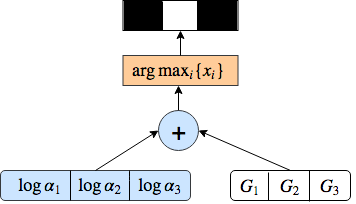
\includegraphics[width=.75\linewidth]{gumbel-max}
  \caption{Gumbel-max trick}
\end{subfigure}%
\begin{subfigure}{.5\textwidth}
  \centering
  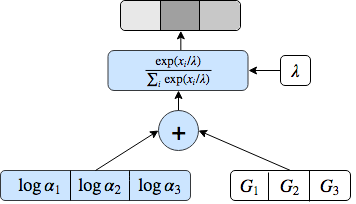
\includegraphics[width=.75\linewidth]{gumbel-softmax}
  \caption{Gumbel-softmax trick}
\end{subfigure}
\caption{Schematics of the Gumbel-max and Gumbel-softmax tricks for 3 random variables. The blue shapes represent the parts of the system that we can and are interested in taking the gradients of. Note how the $\argmax$ operation in orange blocks the gradient, as its output is discrete, whereas the softmax operation relaxes the one-hot representation of the output, depicted as shades of gray instead of black and white, thus permitting gradient flow. Adapted from Maddison et. al. \cite{concrete}}
\label{fig:concrete}
\end{figure}

\bigskip

\noindent This looks promising, as the uniform distribution that we sample from does not depend on any of the parameters of the encoder. However, it is still of no use for our purposes, as we have now introduced a non-continuous $\argmax$ operation. A solution, proposed concurrently by Maddison et. al. \cite{concrete}, and Jang et. al. \cite{gumbel-softmax}, is to approximate it by a softmax function with a tunable temperature parameter $\lambda \in (0, \infty)$, as shown in Equation \ref{eq:gumbel-softmax}. Note that in this case, our sample, drawn from what the authors call a Concrete distribution, is no longer discrete, but rather a continous relaxation of it that approximates a one-hot vector as $\lambda \rightarrow 0$. The difference between the original Gumbel-Max trick, and its Concrete relaxation, sometimes dubbed the Gumbel-Softmax trick, is illustrated in Figure \ref{fig:concrete}.

\begin{equation}
\begin{gathered}
y_i = \frac{\text{exp}((\log \alpha_i + G_i) / \lambda)}{\sum_{j=1}^K \text{exp}((\log \alpha_j + G_j) / \lambda)}.
\end{gathered}
\label{eq:gumbel-softmax}
\end{equation}

\bigskip

\noindent Two additional considerations arise when Concrete variables are used in VAEs. First, since no gradients need to be computed at test time, the distributions can be discretized, allowing real categorical variables to be fed through the graph. Second, the KL term in the objective needs to be modified, as simply "plugging" the continous samples into discrete probability mass functions does not result in a valid KL divergence. This is because the samples are not drawn from the same distribution as is in the enumerator under the logarithm, as shown by Equation \ref{eq:concrete-kl}, where the Concrete posterior is denoted as $q_{\boldsymbol{\alpha}, \lambda}^C$, while $q_{\boldsymbol{\alpha}}$ and $p_{\boldsymbol{\alpha}}$ stand for the approximate categorical posterior and prior, respectively:

\begin{equation}
\begin{gathered}
\mathbb{E}_{\boldsymbol{z} \sim q^{\text{C}}_{\boldsymbol{\alpha}, \lambda}(\boldsymbol{z} | \boldsymbol{x})} \Big[ \log \frac{q_{\boldsymbol{\alpha}}(\boldsymbol{z} | \boldsymbol{x})}{p_{\boldsymbol{\alpha}} (\boldsymbol{z})} \Big].
\end{gathered}
\label{eq:concrete-kl}
\end{equation}

\bigskip

\noindent The authors of the original paper \cite{concrete} provide several options for modifying the KL term, and deem that replacing the discrete masses in the KL with Concrete densitites yields best results. However, unlike the Gaussian case, there is no closed form expression for the KL divergence between two Concrete distributions, so it is necessary to approximate it via sampling. For the types of models considered in this thesis, a variety of estimators, including the one that Maddison et. al. \cite{concrete} advocate, have been found to exhibit too high of a variance, producing poor results as a consequence (Emilien Dupont, personal communication, August 1, 2018). Thus, we opted for replacing the original penalty with an analytic discrete KL term intead:

\begin{equation}
\begin{gathered}
\mathbb{E}_{\boldsymbol{d} \sim q_{\boldsymbol{\alpha}}(\boldsymbol{d} | \boldsymbol{x})} \Big[ \log \frac{q_{\boldsymbol{\alpha}}(\boldsymbol{d} | \boldsymbol{x})}{p_{\boldsymbol{\alpha}} (\boldsymbol{d})} \Big] = \sum_{i=1}^K q_{\boldsymbol{\alpha}}(d_i | \boldsymbol{x}) \log \frac{q_{\boldsymbol{\alpha}}(d_i | \boldsymbol{x})}{p_{\boldsymbol{\alpha}}(d_i)},
\end{gathered}
\label{eq:analytic-discrete-kl}
\end{equation}

\bigskip

\noindent where the vector $\boldsymbol{d}$ represents the one-hot categorical variable. While this strategy provides good results empirically, it is important to emphasize that the use of this KL term in the VAE objective does not necessarily result in a lower-bound of the marginal log-likelihood.

\section{Disentangled representations}

\noindent According to Bengio et. al. \cite{bengio-representation}, a representation is disentangled if it separates explanatory sources of the data into different dimensions (e.g. units) in the latent space. Learning such a representation in an unsupervised manner is challenging, as there is no obvious mathematical objective to optimize. Indeed, the issue is akin to the chicken-and-egg problem, since one would seemingly need to be already aware of the main factors of variation to be able to distill them from the data into the model. \\

\noindent Most earlier work on learning disentangled representations has thus tackled the problem with weakly supervised methods, which require some a-priori knowledge of the data generating factors \cite{transforming-ae, reed2014, yang2016}. DC-IGN \cite{dcign} is perhaps the most well-known method among such approaches. It adopts a clever curriculum learning \cite{bengio-curriculum} strategy to encode the data generating factors into a small subset latent variables in a VAE, each of which is a-priori assigned a symbolic interpretation. During training, a random latent from this predefined group is chosen per each mini-batch of training data, which in turn is carefully constructed such that all training examples in it would vary in only the chosen factor. Finally, the bottleneck layer of the underlying VAE is regularized to indeed only capture all the variance in the current batch with a single latent. \\

\noindent A particularly interesting approach that requires no supervision is Shmidhuber's predictability minimization \cite{pred-min-schmidhuber}. It introduces additional submodules for each unit in an autoencoder's bottleneck layer which try to predict the unit from the remaining ones. In turn, the model is is concurrently optimized to minimize the predictability of the units. The scheme was motivated by the idea that such a minimax game would give rise to an internal representation where each dimension is statistically independent of the others. While this 'competitive learning' framework was indeed found to be able to learn such factorial codes on toy binary datasets, it has not been shown to be able to scale up to more complicated inputs. \\

\noindent The first scalable, purely unsupervised method that showed reasonable level of disentanglement on real-world datasets was InfoGAN, proposed by Chen et. al. \cite{infogan}. They extended the powerful generative adversarial network (GAN) framework \cite{gan} with an additional objective, which would encourage the information between a small subset of the input noise variables and the generated output to be maximized. In practice, this was achieved by adding an additional auxiliary network into the system. The subnetwork, optimized concurrently with the original GAN objective, was fed with the generated images, and tasked to predict the values of a subset of the noise variables that gave rise to it. Contextually, InfoGAN can be seen as a close cousin of both DC-IGN and predictability minimization, borrowing the idea that only a subset of latents should be interpretable from the former, while having an additional subnetwork that predicts the latent activations is akin to the approach of the latter. \\

\noindent The work most relevant to this thesis is that of Higgins et. al. \cite{beta-vae}, which demonstrated that simply adding more weight to the KL term in the VAE objective function encourages the posterior to become disentangled. In particular, they multiplied the divergence measure by a constant $\beta > 1$, giving the model its name, $\beta$-VAE:
\begin{equation}
\begin{gathered}
\mathcal{L}(\boldsymbol{x}; \boldsymbol{\theta}, \boldsymbol{\phi}) =
\mathbb{E}_{\boldsymbol{z} \sim q_{\boldsymbol{\phi}}(\boldsymbol{z}|\boldsymbol{x})} \big[ \log p_{\boldsymbol{\theta}} (\boldsymbol{x} | \boldsymbol{z}) \big] - \beta \, \mathcal{D}_\text{KL}(q_{\boldsymbol{\phi}}(\boldsymbol{z}|\boldsymbol{x}) || p_{\boldsymbol{\theta}}(\boldsymbol{z})).
\end{gathered}
\label{eq:beta-vae}
\end{equation}

\bigskip
\noindent The method superseded InfoGAN, proving to be superior in disentangling, as well as enjoying better training stability. The use of GANs as a backbone has proved to be prohibitive for InfoGAN, as they are notorious for their extremely unstable behaviour in training. Adding further complications, vanilla GANs do not optimize an explicit density function, making it hard to measure the training progress quantitatively \cite{gan-tutorial}. While some recent works have addressed these problems with some success \cite{wgan, wgan-gp, began}, Kim et. al. \cite{factor-vae} found that pluggin them into the InfoGAN framework gives inconsistent results. As $\beta$-VAE uses a principled likelihood-based approach in place of a minimax game whose solution lies at a saddle point in a high-dimensional space, its training dynamics are much more wiedly. \\

\noindent In a closely related follow up work to $\beta$-VAE, Burgess et. al. \cite{understanding-beta-vae} built upon it by proposing an enhanced optimization scheme based on some well-developed intuitive arguments. They analysed the $\beta$-VAE objective via the lens of the information bottleneck principle \cite{tishby-ib}. The principle posits that a good internal representation $Z$ of a learning system is one which is maximally informative about the output $Y$, while also compressing the information in the input $X$. Mathematically, this intuition is expressed as maximizing a Lagrangian, where "informativeness" is naturally measured by mutual information, denoted as $I(\cdot; \cdot)$:
\begin{equation}
\begin{gathered}
\max \big[ I(Z; Y) - \beta I(X;Z) \big]
\end{gathered}
\label{eq:ib}
\end{equation}

\bigskip

\noindent Taking this information-theoretic view of the variational autoencoder, we can conceptualize the probabilistic encoder parameterizing a diagonal Gaussian $q(\boldsymbol{z}|\boldsymbol{x})$ as an independent set of noisy channels $\{z_i\}$, each transmitting information about the input $\boldsymbol{x}$. Accordingly, the KL divergence in Equation \ref{eq:beta-vae} can be thought of as the maximum capacity of said channels per data sample. When the posterior collapses to a unit Gaussian prior $p(\boldsymbol{z})$, the KL term vanishes, and no information about the input is let through the latent bottleneck. Armed with this intuitive framework, it is interesting to analyse how does the reconstruction loss of VAE influence the development of the latent channels. \\

\begin{figure}[H]
\begin{center}
\includegraphics[width=0.3\textwidth,natwidth=215,natheight=297]{understanding-bvae}
\caption{A schematic that illustrates why a VAE is pressured to preserve the locality of inputs in the latent space. If the parmeters of $q(\boldsymbol{z} | \boldsymbol{x}_1)$ are close to that of $q(\boldsymbol{z} | \boldsymbol{x}_2)$, as depicted by the overlapping circles labelled $\boldsymbol{\mu_1}$ and $\boldsymbol{\mu_2}$, a latent $\boldsymbol{z}$ could be sampled such that $\mathcal{N}(\boldsymbol{x}_2|\boldsymbol{\mu_{x|z}}, \boldsymbol{\Sigma_{x|z}}) > \mathcal{N}(\boldsymbol{x}_1|\boldsymbol{\mu_{x|z}}, \boldsymbol{\Sigma_{x|z}})$. Intuitively, this can be thought of as reconstructing the "wrong" datapoint, a mistake whose cost is proportional to the distance between the original and "wrong" datapoint in pixel space.}
\label{fig:understanding-bvae}
\end{center}
\end{figure}

\noindent Burgess et. al. \cite{understanding-beta-vae} argue that trading off the two terms in the $\beta$-VAE objective encourages an encoder to be learned which would have the property that nearby points in data space are close together in the latent space as well. Indeed, suppose that two very different datapoints (as measured by the L2 norm) in pixel-space have similar representations in the latent space. As random noise that is injected into the bottleneck layer, it is likely that the two codes get "mixed up", resulting in the decoder reconstructing the wrong input and incurring a high loss. The situation is illustred in Figure \ref{fig:understanding-bvae}. To avoid such a scenario, we would like the encoding of each datapoint to be as far from others' encodings as possible, which is achieved by squeezing the posterior variances and dispersing their means across datapoints. This, however, is in turn discouraged by the KL penalty term, which pressures the channels to be overlapping for all datapoints. A reasonable compromise between these two opposing forces would be an arrangmenet where the latent space is such that when we do make the occasional mistake of decoding the wrong datapoint, we are at least outputting something that is not too far from the original. \\

\noindent A second fundamental observation Burgess et. al. \cite{understanding-beta-vae} make is that when the latent channel capacities are constrained to be very low, the only information that gets through the bottleneck is one whose utilization by the decoder increases the value of the reconstruction term $\mathbb{E}_{\boldsymbol{z} \sim q_{\boldsymbol{\phi}}(\boldsymbol{z}|\boldsymbol{x})} \big[ \log p_{\boldsymbol{\theta}} (\boldsymbol{x} | \boldsymbol{z}) \big]$ the most. As an example, suppose we have a dataset of white shapes drawn on a black canvas, each of which is has 5 factors of variation: translation along the vertical and horizontal axes, scale, oritentation, and class (heart, square, or ellipse) \cite{dsprites17}. Now, for a high value of $\beta$, only positional information of the sprite might get through the overly constrained latent bottleneck, as getting the position wrong incurs the most cost in terms of log-likelihood. Subsequently, by gradually increasing the capacities of the latent channels, the model starts to allocate additional latents to new factors of variation, like scale and rotation. Crucially, due to the data locality pressure described before, all the factors of variation are encoded into distinct latents, satisfying our working definition of disentanglement. Figure \ref{fig:dsprites-trav} illustrates this phenomenon. \\

\begin{figure}[H]
\begin{center}
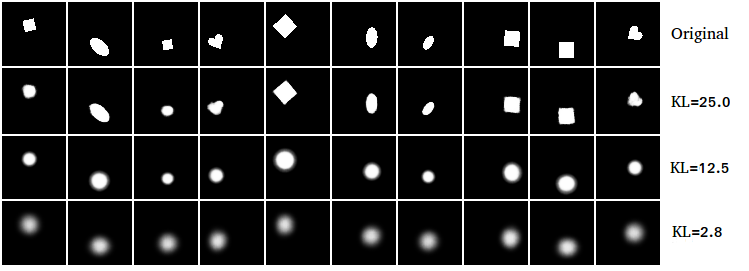
\includegraphics[width=0.6\textwidth,natwidth=749,natheight=271]{gradual-encoding}
\caption{A gradual encoding of data generative factors into the latents on the dSprites dataset \cite{dsprites17} for randomly chosen datapoints. At the start of training, when the capacities of the latent channels are kept low, only the x and y positions of the sprites is encoded (bottom row). Next, as capacity is increased, the size of the sprite is captured (third row). Finally, the rotation and class of the figure is discovered (second row).}
\label{fig:dsprites-trav}
\end{center}
\end{figure}

\noindent The intuitive framework laid out above suggests a natural modification to the $\beta$-VAE objective, given by Equation \ref{eq:cc-vae}. In the new formulation, the capacities of the channels, denoted as $C$, are made explicit, and increased gradually in the course of training. The new hyperparameter $\gamma$ specifies the degree of pressure put on the latent channels to be close to their desired capacity. It is usually chosen big enough that the KL term would be relatively close to $C$ at all times, as this makes the external control of the channel capacities rather convenient.

\begin{equation}
\begin{gathered}
\mathcal{L}(\boldsymbol{x}; \boldsymbol{\theta}, \boldsymbol{\phi}) =
\mathbb{E}_{\boldsymbol{z} \sim q_{\boldsymbol{\phi}}(\boldsymbol{z}|\boldsymbol{x})} \big[ \log p_{\boldsymbol{\theta}} (\boldsymbol{x} | \boldsymbol{z}) \big] - \gamma \, | \mathcal{D}_\text{KL}(q_{\boldsymbol{\phi}}(\boldsymbol{z}|\boldsymbol{x}) || p_{\boldsymbol{\theta}}(\boldsymbol{z})) - C |.
\end{gathered}
\label{eq:cc-vae}
\end{equation} 

\bigskip

\noindent While $\beta$-VAE with a controlled capacity increase showed good results disentangling continuous factors of variation, it struggled to capture discrete generative factors. For example, it was unable to disentangle the individual classes in the MNIST handwritten digits dataset. As a way to overcome this difficuly, Dupont introduced JointVAE \cite{joint-vae}, which augmented the original multivariate normal latent distirbution of $\beta$-VAE with categorical Concrete random variables, leading to the following objective:

\begin{equation}
\begin{gathered}
\mathcal{L}(\boldsymbol{x}; \boldsymbol{\theta}, \boldsymbol{\phi}) =
\mathbb{E}_{\boldsymbol{z, c} \sim q_{\boldsymbol{\phi}}(\boldsymbol{z, c}|\boldsymbol{x})} \big[ \log p_{\boldsymbol{\theta}} (\boldsymbol{x} | \boldsymbol{z, c}) \big] - \\ \gamma \big\{ | \mathcal{D}_\text{KL}(q_{\boldsymbol{\phi}}(\boldsymbol{z}|\boldsymbol{x}) || p_{\boldsymbol{\theta}}(\boldsymbol{z})) - C_z | + | \mathcal{D}_\text{KL}(q_{\boldsymbol{\phi}}(\boldsymbol{c}|\boldsymbol{x}) || p_{\boldsymbol{\theta}}(\boldsymbol{c})) - C_c | \big\},
\end{gathered}
\label{eq:joint-vae}
\end{equation}

\bigskip

\noindent where $\boldsymbol{z}$ and $\boldsymbol{c}$ denote the continous Gaussian and Concrete latent variables, respectively. The new model was shown to be able to outperform the original formulation of $\beta$-VAE on datasets where capturing discrete generative factors is paramount to achieving good reconstruction quality, as is the case for MNIST. However, complete disentanglement of the sprites dataset is still beyond the capabilities of current models, as the types of shapes are all quite similar in terms of the area they cover, making the possible increase in log-likelihood marginal.

\section{Adversarial examples}

\noindent The problem of adversarial examples in the context of deep neural networks was first articulated by Szegedy et. al. \cite{intriguing-properties}. They showed that by perturbing the pixels of the input image by an (almost) imperceptibly small amount, it is possible to cause neural-network based classifiers to assign high likelihoods to arbitrary classes. It is important to stress that the pixels of the original image are not changed randomly, but are rather done so in a principled way. More specifically, the authors use box-constrained L-BFGS \cite{NoceWrig06} to solve the following optimization problem \footnote{Note that this specific formulation constrains the images to have a single channel and either be normalized or grayscale. However, generalizing it to unnormalized RGB images is straightforward.}:

\begin{equation}
\begin{aligned}
\text{minimize } &c \Vert \boldsymbol{r} \Vert_2 + \text{loss}_f(\boldsymbol{x}+\boldsymbol{r}, l) \\
\text{subject to } &\boldsymbol{x} + \boldsymbol{r} \in [0, 1]^m,
\end{aligned}
\label{eq:adv-class-opt}
\end{equation}

\bigskip

\noindent where $\boldsymbol{r}$ is the m-dimensional perturbation vector that is added to the original image $\boldsymbol{x}$, such that the classifier $f$ would output the class $l$. $\text{loss}_f$ is some continuous measure of classification loss, commmonly taken to be cross-entropy, while the coefficient $c > 0$ balances the the size of the perturbation and the loss for the generated adversarial image. Of course, the problem is only of interest when $f(\boldsymbol{x}) \neq l$. Figure \ref{fig:adversarial-cls} illustrates some adversarial examples $\boldsymbol{x}$ + $\boldsymbol{r}$ generated by this procedure.

\bigskip

\begin{figure}[H]
\begin{center}
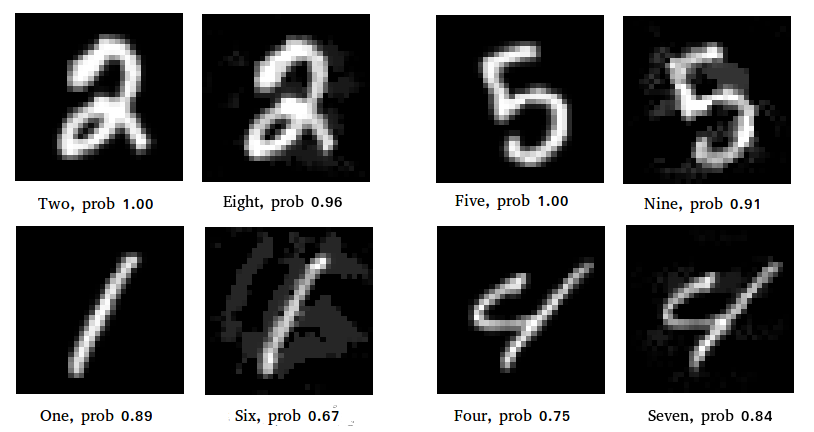
\includegraphics[width=0.6\textwidth,natwidth=814,natheight=271]{adversarial-cls}
\caption{Adversarial examples for the MNIST handwritten digits dataset. The left image of each pair depicts the original, correctly classified image. The right image, however, is the adversarial input, derived from the original, that fools the classifier.}
\label{fig:adversarial-cls}
\end{center}
\end{figure}

\noindent In subsequent work, Goodfellow et. al. \cite{explaining-and-harnessing} argue that the existence of adversarial examples can be at least partially explained by the linear nature of the underlying classifiers. Linear models have the property that their outputs change proportionally to the change in the intensity of any of the pixels. Thus, given an input with high enough dimensionality, one can make small perturbtions to a large number of pixels, all of which add up to produce a large shift in the output. Goodfellow et. al. make the observation that this same phenomenon can manifest itself in modern deep neural networks, as they are often explicitly constructed to be rather linear for ease of optimization. Illustrative examples include the rectified linear units as general-purpose activation functions \cite{relu}, LSTMs for time-series analysis \cite{lstm}, and residual networks for compute vision \cite{resnet}. Moreover, adding further evidence in favour of the linearity hypothesis, they observed that RBF networks \cite{rbf-networks} - a method that classifies inputs based on their similarity (as measured by the exponentiated quadratic kernels) to a set of predefined centroids - are significantly more robust to adversarial examples. \\

\noindent One of the most surprising properties of adversarial examples is their generality and transferability. Early work on the problem found that they generalize across different partitions of the same dataset \cite{intriguing-properties} and across models with different architectures \cite{explaining-and-harnessing}. More recently, Kurakin. et. al. \cite{kurakin16} discovered that they can also be extrapolated to the physical world, showing that models trained on the regular ImageNet \cite{imagenet} dataset are misclassifying adversarial examples even if they are printed on paper and viewed through a physical camera. Somewhat reassuringly, they have also been found to fool time-limited humans \cite{humans-adv}. While most research on adversarial examples has focussed on image classification, models trained to solve other kinds of machine learning tasks are subject to them as well, including ones specializing in speech-to-text \cite{audio-adv}, neural machine translation \cite{nmt-adv}, and deep reinforcement learning \cite{rl-adv}. \\

\noindent Pertinent to this thesis is the work of Kos. et. al. \cite{kos-gen-adv}, who investigate adversarial examples in the context of generative models. They found that VAEs and VAE-GANs \cite{vaegan}, a derivative of VAEs which enjoys better sample quality due to the fact that its reconstruction loss operates in the feature space of a GAN, are also suspect to them. To generate adversarial examples for such models, they took inspiration from Sabour et. al. \cite{sabour}, and perturbed the source image in such a way that its predicted posterior mean would be close to the posterior mean of some target image. Mathematically, this optimization problem is equivalent to the one in Equation \ref{eq:adv-class-opt}, with the classification loss replaced by the L2 norm measuring the discrepancy of the latent representations. They did, however, use Adam instead of L-BFGS for optimization, as advocated by Carlini \& Wagner \cite{carlini-wagner-16}. \\

\noindent Another relevant work from our point of view is that of Alemi et. al. \cite{deep-variational-bottleneck}, in which they parameterize the information bottleneck in Equation \ref{eq:ib} using neural networks. By subsequently deriving a variational lower bound to this objective and making use of the reparatemerization trick, they end up with a model anologus to that of $\beta$-VAE, given that the output variable $Y$ in Equation \ref{eq:ib} is taken to be the reconstruction of the input. However, as their treatment is more broad, they are also able to generalize this approach to a classification setting, by taking $Y$ to be the class label. Intuitively, this amounts to swapping the decoder of $\beta$-VAE with an appropriate classifier. To demonstrate the usefulness of the bottleneck principle, they measured the robustness of the resulting classifier to adversarial examples on the MNIST and ImageNet datasets. They found that the model becomes progressively harder to fool as the capacity of the bottleneck is increased.

\chapter{Methods}

\noindent We used the MNIST handwritten digits dataset to measure the effect that a disentangled representation has on the ability to generate adversarial examples for VAEs. The dataset consists of $70,000$ images (partitioned into a train-eval-test split of $50,000$, $10,000$ and $10,000$ datapoints, respectively), each of which is assigned to a numeric class from 0 to 9. MNIST is one of the few datasets that have been extensively analysed both in the disentanglement, as well as in the adversarial example literature. It was the first dataset for which adversarial examples were constructed \cite{intriguing-properties}, and it has been shown that at least 3 factors of variation of handwritten digits can be disentangled on this dataset: class, angle, and thickness \cite{infogan}, \cite{joint-vae}. Moreover, the two most closely related works to this thesis, that of Kos et. al. and Alemi et. al., concentrate on MNIST as well, making drawing comparisons easier. \\

\noindent We also experimented with generating adversarial examples for other datasets, including dSprties and CelebA, a large-scale dataset of celebrety faces \cite{celeba}. Unfortunately, we found that dSprites is not sensitive to adversarial examples in the generative setting. This phenomenon is possibly due to the relatively simple visual appearance of the datapoints, resulting in 2 different inputs to have a relatively sparse set of common features that could be made use of while generating an adversarial input. Similarly, for CelebA, we were unable to construct adversarial examples with enough visual fidelity that would permit reasonable quantitative analysis to be carried out. \\

\noindent As our disentangled model, we used JointVAE \cite{joint-vae}, an equivalent model to $\beta$-VAE, but with both continuous and discrete (or Concrete) latent variables, whose channel capacities were gradually increased during training. A regular VAE without any regularization was taken to be a baseline. However, as decreasing the capacity of the latent channels constrains the amount of information that gets through the bottleneck, the reconstructions produced by JointVAE are somewhat worse than that of a regular VAE. In order to account for that effect, we also trained a second baseline model, which was regularized using weight-decay and achieved similar reconstruction quality as our disentangled model. All 3 trained models had the same architecture as was used by Dupont \cite{joint-vae}, outlined in Table \ref{tab:architecture}. \\

\begin{center}
\begin{tabular}{|l|l|}
\hline
\textbf{Encoder} & \textbf{Decoder} \\ \hline
\text{$\boldsymbol{x} \in \mathbb{R}^{32\times32}$ grayscale image} & \text{$\boldsymbol{z} \in \mathbb{R}^{20}$} \\ \hline
\text{Conv 4$\times$4. 32 ReLU, 2 stride} & Dense. 128 ReLU \\ \hline
\text{Conv 4$\times$4. 32 ReLU, 2 stride} & Dense. 64$\times$4$\times$4 ReLU \\ \hline
\text{Conv 4$\times$4. 64 ReLU, 2 stride} & Upconv 4$\times$4. 64 ReLU, 2 stride \\ \hline
\text{Dense. 128 ReLU} & Upconv 4$\times$4. 32 ReLU, 2 stride \\ \hline
\text{Dense. 20 linear} & Upconv 4$\times$4. 32 sigmoid, 2 stride \\ \hline
\end{tabular}
\captionof{table}{VAE architecture used for the experiments carried out in this work. The bottleneck layer parameterized a 10-dimensional diagonal multivariate normal distribution, as well as a 10-way categorical Concrete distribution, which results in a 20-dimensional latent vector to be fed into the decoder.}\label{tab:architecture}
\end{center}

\noindent All models were trained with the Adam optimizer with a constant learning rate of $0.0001$ for $100,000$ randomly chosen batches from the training set with a mini-batch size of $64$. Following the guidelines of Maddison et. al. \cite{concrete} \footnote{They show that at temperatures lower than $(n-1)^{-1}$, where $n$ is the dimensionality of the Concrete variable, the probability simplex corresponding to the Concrete distribution is guaranteed not to have any modes in its interior. This gives us some confidence that our continuous relaxation is not too far from the corresponding discretized variable.}, the temperature parameter for the 10-way categorical Concrete distribution was taken to be $0.1$. For JointVAE, the initial latent capacities for both the continuous and discrete KL terms ($C_z$ and $C_c$ in in Equation \ref{eq:joint-vae}, respectively) were taken to be 0, which were linearly increased to $5$ over the whole training procedure. The capacity coefficient $\gamma$ for FactorVAE was taken to be $30$, which ensured that the KL was close to its target value at all times. The weight-decay coefficient for VAE with L2 regularization was chosen to be $0.5$. \\

\noindent To generate adversarial examples for the preceding models, we used the latent-attack methodology of Kos et. al. \cite{kos-gen-adv}. In particular, the optimization problem in Equation \ref{eq:adv-gen} is solved with the Adam optimizer for $1000$ steps, with a learning rate of $0.001$ and a relative weighting coefficient $\lambda = 1$.

\begin{equation}
\begin{aligned}
\argmin_{\boldsymbol{x}_{*}} \text{ } &\lambda \Vert \boldsymbol{x}_s - \boldsymbol{x}_{*} \Vert_2 + \Vert [\boldsymbol{\mu}_t, \boldsymbol{\alpha}_t]^T - [\boldsymbol{\mu}_{*}, \boldsymbol{\alpha}_{*}]^T \Vert_2 \\ 
\text{subject to } &\boldsymbol{x_{*}} \in [0, 1]^m,
\end{aligned}
\label{eq:adv-gen}
\end{equation}

\bigskip

\noindent where $\boldsymbol{x}_s$ is the original $m$-dimensional source image, $\boldsymbol{\mu}_t$ represents the approximate posterior mean of the target image which we are trying to adversarially reconstruct, $\boldsymbol{\alpha}_x$ represents the logits of the target's latent Concrete distribution, and $\boldsymbol{\mu}_*$, $\boldsymbol{\alpha}_*$ represent the same quantities, but for the adversarial image $\boldsymbol{x}_{*}$. \\

\noindent Following Kos et. al. \cite{kos-gen-adv}, a classifier, trained to recognize the types of MNIST digits, was used to derive two metrics for quantifying the effectiveness of the attacks. The model, whose arcitecture is outlined in Table \ref{tab:cls-arch}, was trained with momentum-based stochastic gradient descent for $10$ epochs on the MNIST training set with a batch size of $64$. After training, it achieved a test set accuracy of $98\%$. 

\begin{center}
\begin{tabular}{|l|}
\hline
\textbf{Classifier} \\ \hline
\text{$\boldsymbol{x} \in \mathbb{R}^{32\times32}$ grayscale image} \\ \hline
\text{Conv 5$\times$5. 10 ReLU, 1 stride} \\ \hline
\text{Maxpool 2$\times$2. 2 stride} \\ \hline
\text{Conv 5$\times$5. 10 ReLU, 1 stride} \\ \hline
\text{Maxpool 2$\times$2. 2 stride} \\ \hline
\text{Dropout (p=0.5)} \\ \hline
\text{Dense. 50 ReLU} \\ \hline
\text{Dense. 10 softmax} \\ \hline
\end{tabular}
\captionof{table}{Architecture of a simple MNIST classifier.}\label{tab:cls-arch}
\end{center}

\bigskip

\noindent The first metric, $AS_{\text{ignore-target}}$ measures the adversarial example's ability to reconstruct an image that depicts a digit that is different from that of the source image. Under this metric, an attack is successful even if the reconstructed digit has a different class than the source image \textit{and} the target image. \todo{More\dots} \\

\noindent The second metric, $AS_{\text{target}}$ \dots \todo{More\dots} \\

\noindent Suppose the MNIST test set is partitioned into 9 disjoint subsets, with  subset $S_j$ containing the images corresponding to class $j$, with $j = 0, 1, \dots, 9$. For each image $\boldsymbol{x}$ belonging to class $i$ in the MNIST test set, a random example $\boldsymbol{x}_j$ was drawn from each of the partitions $S_j$, $j \neq i$. The $9$ adversarial attacks were then carried out with $\boldsymbol{x}$ as source and $\boldsymbol{x}_j$ as targets. The generated adversarial examples were then fed into the MNIST classifier 

\noindent Following Kos et. al. \cite{kos-gen-adv}, two metrics were used to derive attack effectiveness 

\chapter{Results}

\begin{figure}
\begin{center}
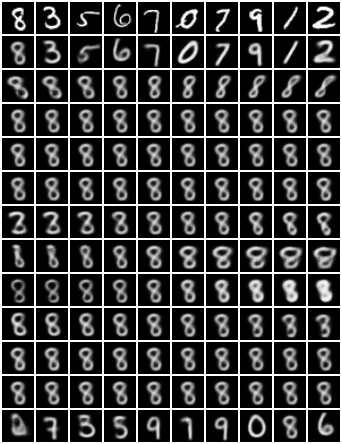
\includegraphics[width=0.5\textwidth,natwidth=342,natheight=342]{mnist_dis_trav}
\end{center}
\caption{mnist disentangled traversal}
\end{figure}

\begin{figure}
\begin{center}
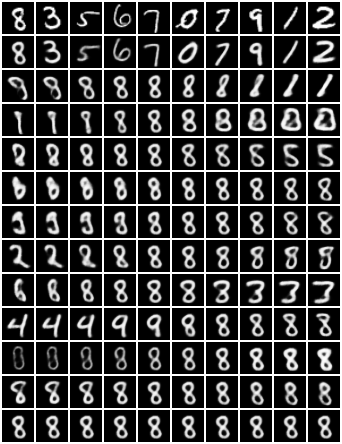
\includegraphics[width=0.5\textwidth,natwidth=342,natheight=342]{mnist_ent_trav}
\end{center}
\caption{MNIST entangled reconstruction}
\end{figure}

\begin{figure}
\begin{center}
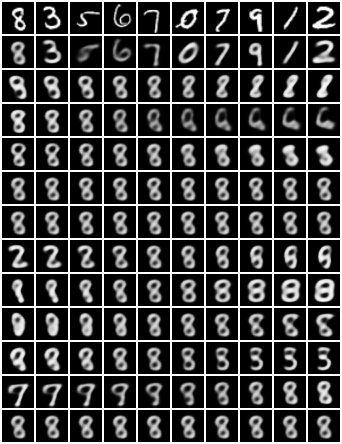
\includegraphics[width=0.5\textwidth,natwidth=342,natheight=342]{mnist_ent_wdec_trav}
\end{center}
\caption{MNIST entangled weight decay reconstruction}
\end{figure}

\begin{figure}
\begin{subfigure}{.5\textwidth}
  \centering
  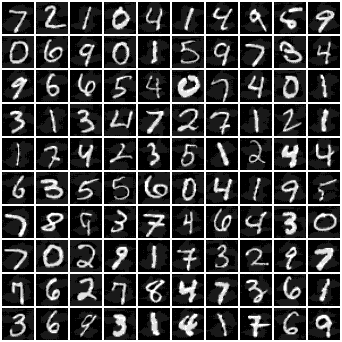
\includegraphics[width=.9\linewidth]{mnist_dis_advs}
  \caption{adv}
\end{subfigure}%
\begin{subfigure}{.5\textwidth}
  \centering
  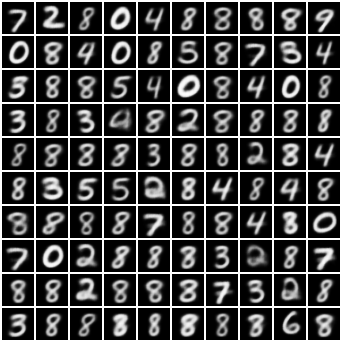
\includegraphics[width=.9\linewidth]{mnist_dis_adv_recons}
  \caption{adv recon}
\end{subfigure}
\caption{MNIST disentangled adv and adv recon}
\label{fig:mnist-dis-advs}
\end{figure}

\begin{figure}
\begin{subfigure}{.5\textwidth}
  \centering
  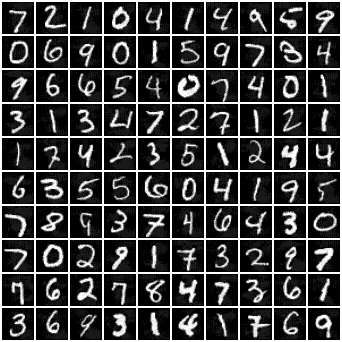
\includegraphics[width=.9\linewidth]{mnist_ent_advs}
  \caption{adv}
\end{subfigure}%
\begin{subfigure}{.5\textwidth}
  \centering
  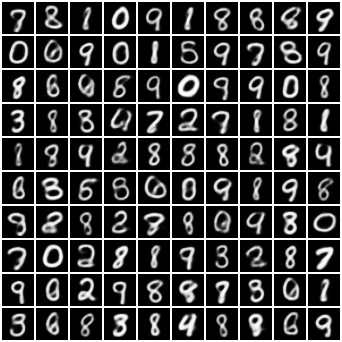
\includegraphics[width=.9\linewidth]{mnist_ent_adv_recons}
  \caption{adv recon}
\end{subfigure}
\caption{MNIST ent adv and adv recon}
\label{fig:mnist-ent-advs}
\end{figure}

\begin{center}
  \begin{tabular}{|c|c|c|}
  \hline
   & \textbf{AS ignore-target} & \textbf{AS target} \\ \hline
  \textbf{Disentangled} & 36.86\% & 12.54\% \\ \hline
  \textbf{Entangled} & 29.83\% & 9.49\% \\ \hline
  \textbf{Entangled wdec} & 26.88\% & 7.85\% \\ \hline
  \end{tabular}
\captionof{table}{Means}
\end{center}

\begin{center}
{\tiny
  \begin{tabular}{c|c|c|c|c|c|}
  \hline
  \multicolumn{1}{|c|}{\textbf{Source}} & \textbf{0} & \textbf{1} & \textbf{2} & \textbf{3} & \textbf{4}\\ \hline
  \multicolumn{1}{|c|}{\textbf{Disentangled}} & \cellcolor{light-gray} \makecell{8.89\% \\ (3.18\%)} & \cellcolor{light-gray} \makecell{82.62\% \\ (33.76\%)} & \cellcolor{light-gray} \makecell{20.92\% \\ (5.36\%)} & \cellcolor{light-gray} \makecell{16.72\% \\ (6.20\%)} & \makecell{33.73\% \\ (13.02\%)} \\ \hline
  \multicolumn{1}{|c|}{\textbf{Entangled}} & \makecell{6.12\% \\ (1.93\%)} & \makecell{63.75\% \\ (28.58\%)} & \makecell{11.12\% \\ (3.06\%)} & \makecell{12.11\% \\ (4.30\%)} & \cellcolor{light-gray} \makecell{64.40\% \\ (13.46\%)} \\ \hline
  \multicolumn{1}{|c|}{\textbf{Entangled wdec}} & \makecell{3.30\% \\ (0.97\%)} & \makecell{59.78\% \\ (23.44\%)} & \makecell{7.09\% \\ (1.41\%)} & \makecell{10.83\% \\ (3.02\%)} & \makecell{53.99\% \\ (10.94\%)} \\ \hline
  & \textbf{5} & \textbf{6} & \textbf{7} & \textbf{8} & \textbf{9} \\ \cline{2-6}
  & \cellcolor{light-gray} \makecell{44.25\% \\ (11.24\%)} & \cellcolor{light-gray} \makecell{38.49\% \\ (13.48\%)} & \cellcolor{light-gray} \makecell{40.57\% \\ (11.65\%)} & \makecell{18.23\% \\ (8.47\%)} & \cellcolor{light-gray} \makecell{64.23\% \\ (18.97\%)} \\ \cline{2-6}
  & \makecell{37.79\% \\ (11.04\%)} & \makecell{27.83\% \\ (9.55\%)} & \makecell{39.70\% \\ (7.89\%)} & \makecell{16.27\% \\ (6.43\%)} & \makecell{19.19\% \\ (8.70\%)} \\ \cline{2-6}
  & \makecell{34.74\% \\ (8.65\%)} & \makecell{24.94\% \\ (6.10\%)} & \makecell{18.45\% \\ (4.26\%)} & \cellcolor{light-gray} \makecell{23.46\% \\ (7.61\%)} & \makecell{32.28\% \\ (12.09\%)} \\ \cline{2-6}
  \end{tabular}
}
\captionof{table}{Source marginals}
\end{center}

\begin{center}
{\tiny
  \begin{tabular}{c|c|c|c|c|c|}
  \hline
  \multicolumn{1}{|c|}{\textbf{Target}} & \textbf{0} & \textbf{1} & \textbf{2} & \textbf{3} & \textbf{4} \\ \hline
  \multicolumn{1}{|c|}{\textbf{Disentangled}} & \cellcolor{light-gray} \makecell{40.36\% \\ (1.78\%)} &  \cellcolor{light-gray} \makecell{25.91\% \\ (0.93\%)} &  \cellcolor{light-gray} \makecell{46.50\% \\ (25.91\%)} & \cellcolor{light-gray} \makecell{41.81\% \\ (10.19\%)} & \cellcolor{light-gray} \makecell{31.76\% \\ (14.23\%)} \\ \hline
  \multicolumn{1}{|c|}{\textbf{Entangled}} & \makecell{29.39\% \\ (3.52\%)} & \makecell{13.88\% \\ (0.24\%)} & \makecell{35.42\% \\ (11.50\%)} & \makecell{40.39\% \\ (18.68\%)} & \makecell{24.71\% \\ (5.53\%)} \\ \hline
  \multicolumn{1}{|c|}{\textbf{Entangled wdec}} & \makecell{28.36\% \\ (4.50\%)} & \makecell{12.62\% \\ (1.06\%)} & \makecell{37.50\% \\ (16.60\%)} & \makecell{36.40\% \\ (12.30\%)} & \makecell{19.14\% \\ (1.88\%)} \\ \hline
  & \textbf{5} & \textbf{6} & \textbf{7} & \textbf{8} & \textbf{9} \\ \cline{2-6}
  & \cellcolor{light-gray} \makecell{38.98\% \\ (10.04\%)} & \cellcolor{light-gray} \makecell{37.46\% \\ (7.80\%)} & \makecell{27.77\% \\ (7.42\%)} & \cellcolor{light-gray} \makecell{46.23\% \\ (32.19\%)} & \cellcolor{light-gray} \makecell{31.87\% \\ (14.87\%)} \\ \cline{2-6}
  & \makecell{32.75\% \\ (7.38\%)} & \makecell{22.94\% \\ (4.23\%)} & \cellcolor{light-gray} \makecell{28.20\% \\ (4.54\%)} & \makecell{43.49\% \\ (25.44\%)} & \makecell{27.11\% \\ (13.87\%)} \\ \cline{2-6}
  & \makecell{27.39\% \\ (4.44\%)} & \makecell{20.63\% \\ (3.89\%)} & \makecell{29.92\% \\ (12.57\%)} & \makecell{33.21\% \\ (12.55\%)} & \makecell{23.67\% \\ (8.72\%)} \\ \cline{2-6}
  \end{tabular}
}
\captionof{table}{Target marginals}
\end{center}

\chapter{Conclusion}

\chapter{Appendix}

\begin{table}
\noindent\makebox[\textwidth]{
{\tiny
  \begin{tabular}{|c|c|c|c|c|c|c|c|c|c|c|}
  \cline{1-11}
  \multirow{2}{*}{\textbf{Source}}
  & \multicolumn{10}{|c|}{\textbf{Targets}}  \\ \cline {2-11}
  & \textbf{0} & \textbf{1} & \textbf{2} & \textbf{3} & \textbf{4} & \textbf{5} & \textbf{6} & \textbf{7} & \textbf{8} & \textbf{9}  \\ \hline
  \textbf{0} & - & \makecell{6.58\% \\ (0.00\%)} & \makecell{11.12\% \\ (5.98\%)} & \makecell{8.36\% \\ (3.34\%)} & \makecell{9.21\% \\ (1.99\%)} & \makecell{11.15\% \\ (6.44\%)} & \makecell{8.13\% \\ (4.71\%)} & \makecell{7.60\% \\ (0.31\%)} & \makecell{8.74\% \\ (5.89\%)} & \makecell{9.10\% \\ (0.00\%)} \\ \hline
\textbf{1} & \makecell{99.48\% \\ (0.00\%)} & - & \makecell{97.62\% \\ (93.64\%)} & \makecell{95.63\% \\ (4.98\%)} & \makecell{73.25\% \\ (42.63\%)} & \makecell{95.49\% \\ (10.87\%)} & \makecell{97.64\% \\ (26.85\%)} & \makecell{23.43\% \\ (13.36\%)} & \makecell{95.48\% \\ (72.58\%)} & \makecell{65.52\% \\ (38.95\%)} \\ \hline
\textbf{2} & \makecell{7.74\% \\ (0.66\%)} & \makecell{24.84\% \\ (0.42\%)} & - & \makecell{14.63\% \\ (4.33\%)} & \makecell{27.98\% \\ (4.24\%)} & \makecell{23.36\% \\ (1.58\%)} & \makecell{6.64\% \\ (2.29\%)} & \makecell{26.38\% \\ (12.29\%)} & \makecell{26.85\% \\ (22.36\%)} & \makecell{29.84\% \\ (0.11\%)} \\ \hline
\textbf{3} & \makecell{2.90\% \\ (0.58\%)} & \makecell{20.00\% \\ (1.14\%)} & \makecell{16.61\% \\ (11.86\%)} & - & \makecell{19.27\% \\ (0.80\%)} & \makecell{17.33\% \\ (14.38\%)} & \makecell{12.00\% \\ (1.43\%)} & \makecell{19.86\% \\ (1.47\%)} & \makecell{24.27\% \\ (19.49\%)} & \makecell{18.22\% \\ (4.61\%)} \\ \hline
\textbf{4} & \makecell{24.70\% \\ (0.85\%)} & \makecell{44.48\% \\ (0.48\%)} & \makecell{37.18\% \\ (25.28\%)} & \makecell{31.27\% \\ (8.15\%)} & - & \makecell{21.63\% \\ (4.27\%)} & \makecell{21.31\% \\ (11.65\%)} & \makecell{51.10\% \\ (6.48\%)} & \makecell{34.71\% \\ (26.55\%)} & \makecell{37.16\% \\ (33.50\%)} \\ \hline
\textbf{5} & \makecell{46.66\% \\ (3.54\%)} & \makecell{45.71\% \\ (0.65\%)} & \makecell{67.40\% \\ (8.54\%)} & \makecell{34.48\% \\ (26.92\%)} & \makecell{31.63\% \\ (8.79\%)} & - & \makecell{51.50\% \\ (12.26\%)} & \makecell{42.93\% \\ (2.36\%)} & \makecell{46.55\% \\ (30.24\%)} & \makecell{31.36\% \\ (7.87\%)} \\ \hline
\textbf{6} & \makecell{28.87\% \\ (7.41\%)} & \makecell{34.20\% \\ (2.72\%)} & \makecell{39.89\% \\ (33.11\%)} & \makecell{39.65\% \\ (6.35\%)} & \makecell{38.06\% \\ (24.21\%)} & \makecell{33.49\% \\ (10.85\%)} & - & \makecell{38.18\% \\ (2.74\%)} & \makecell{50.00\% \\ (27.84\%)} & \makecell{44.10\% \\ (6.11\%)} \\ \hline
\textbf{7} & \makecell{47.31\% \\ (1.43\%)} & \makecell{4.44\% \\ (0.23\%)} & \makecell{40.25\% \\ (24.94\%)} & \makecell{47.69\% \\ (2.08\%)} & \makecell{38.66\% \\ (4.94\%)} & \makecell{52.41\% \\ (6.63\%)} & \makecell{41.66\% \\ (0.37\%)} & - & \makecell{49.03\% \\ (27.36\%)} & \makecell{43.71\% \\ (36.91\%)} \\ \hline
\textbf{8} & \makecell{25.11\% \\ (0.79\%)} & \makecell{13.13\% \\ (1.71\%)} & \makecell{30.48\% \\ (24.20\%)} & \makecell{24.06\% \\ (14.71\%)} & \makecell{11.16\% \\ (5.69\%)} & \makecell{18.67\% \\ (12.36\%)} & \makecell{22.80\% \\ (6.02\%)} & \makecell{10.87\% \\ (5.03\%)} & - & \makecell{7.79\% \\ (5.73\%)} \\ \hline
\textbf{9} & \makecell{80.48\% \\ (0.80\%)} & \makecell{39.78\% \\ (1.01\%)} & \makecell{77.94\% \\ (5.65\%)} & \makecell{80.51\% \\ (20.82\%)} & \makecell{36.64\% \\ (34.79\%)} & \makecell{77.28\% \\ (22.97\%)} & \makecell{75.44\% \\ (4.60\%)} & \makecell{29.54\% \\ (22.74\%)} & \makecell{80.48\% \\ (57.39\%)} & - \\ \hline
\end{tabular}
}
}
\captionof{table}{Disentangled}
\end{table}


\begin{table}
\noindent\makebox[\textwidth]{
{\tiny
  \begin{tabular}{|c|c|c|c|c|c|c|c|c|c|c|}
  \cline{1-11}
  \multirow{2}{*}{\textbf{Source}}
  & \multicolumn{10}{ c| }{\textbf{Targets}}  \\ \cline {2-11}
  & \textbf{0} & \textbf{1} & \textbf{2} & \textbf{3} & \textbf{4} & \textbf{5} & \textbf{6} & \textbf{7} & \textbf{8} & \textbf{9}  \\ \hline
  \textbf{0} & - & \makecell{3.46\% \\ (0.00\%)} & \makecell{8.93\% \\ (2.60\%)} & \makecell{7.47\% \\ (1.89\%)} & \makecell{6.85\% \\ (0.31\%)} & \makecell{5.59\% \\ (1.60\%)} & \makecell{5.74\% \\ (2.34\%)} & \makecell{4.58\% \\ (0.42\%)} & \makecell{8.82\% \\ (6.51\%)} & \makecell{3.65\% \\ (1.67\%)} \\ \hline
\textbf{1} & \makecell{58.13\% \\ (0.21\%)} & - & \makecell{76.68\% \\ (52.17\%)} & \makecell{69.11\% \\ (41.26\%)} & \makecell{60.94\% \\ (24.38\%)} & \makecell{66.59\% \\ (17.45\%)} & \makecell{50.53\% \\ (19.64\%)} & \makecell{64.42\% \\ (28.05\%)} & \makecell{73.72\% \\ (55.29\%)} & \makecell{53.65\% \\ (18.76\%)} \\ \hline
\textbf{2} & \makecell{13.13\% \\ (1.89\%)} & \makecell{4.53\% \\ (0.10\%)} & - & \makecell{13.32\% \\ (9.73\%)} & \makecell{9.25\% \\ (0.54\%)} & \makecell{14.37\% \\ (0.36\%)} & \makecell{11.17\% \\ (1.02\%)} & \makecell{7.71\% \\ (1.04\%)} & \makecell{16.65\% \\ (12.13\%)} & \makecell{9.94\% \\ (0.74\%)} \\ \hline
\textbf{3} & \makecell{8.26\% \\ (1.00\%)} & \makecell{4.71\% \\ (0.11\%)} & \makecell{6.93\% \\ (4.01\%)} & - & \makecell{20.51\% \\ (0.11\%)} & \makecell{14.46\% \\ (10.78\%)} & \makecell{12.30\% \\ (0.68\%)} & \makecell{4.75\% \\ (0.22\%)} & \makecell{26.07\% \\ (19.89\%)} & \makecell{11.00\% \\ (1.92\%)} \\ \hline
\textbf{4} & \makecell{65.87\% \\ (3.26\%)} & \makecell{42.55\% \\ (0.65\%)} & \makecell{66.48\% \\ (9.88\%)} & \makecell{89.27\% \\ (10.51\%)} & - & \makecell{79.10\% \\ (4.01\%)} & \makecell{26.20\% \\ (5.15\%)} & \makecell{71.54\% \\ (3.79\%)} & \makecell{79.87\% \\ (30.09\%)} & \makecell{58.75\% \\ (53.80\%)} \\ \hline
\textbf{5} & \makecell{37.52\% \\ (4.06\%)} & \makecell{23.74\% \\ (0.12\%)} & \makecell{49.51\% \\ (6.25\%)} & \makecell{40.81\% \\ (30.51\%)} & \makecell{38.44\% \\ (0.49\%)} & - & \makecell{26.43\% \\ (6.82\%)} & \makecell{33.75\% \\ (0.62\%)} & \makecell{55.09\% \\ (42.21\%)} & \makecell{34.78\% \\ (8.29\%)} \\ \hline
\textbf{6} & \makecell{25.22\% \\ (17.32\%)} & \makecell{6.80\% \\ (0.44\%)} & \makecell{29.56\% \\ (8.57\%)} & \makecell{41.88\% \\ (9.42\%)} & \makecell{14.19\% \\ (6.22\%)} & \makecell{27.86\% \\ (15.47\%)} & - & \makecell{38.40\% \\ (0.33\%)} & \makecell{42.39\% \\ (25.33\%)} & \makecell{24.19\% \\ (2.82\%)} \\ \hline
\textbf{7} & \makecell{33.82\% \\ (1.12\%)} & \makecell{24.40\% \\ (0.21\%)} & \makecell{30.49\% \\ (8.33\%)} & \makecell{28.37\% \\ (12.51\%)} & \makecell{50.22\% \\ (6.47\%)} & \makecell{40.85\% \\ (1.09\%)} & \makecell{55.27\% \\ (0.11\%)} & - & \makecell{56.51\% \\ (9.71\%)} & \makecell{37.35\% \\ (31.43\%)} \\ \hline
\textbf{8} & \makecell{12.83\% \\ (1.03\%)} & \makecell{7.80\% \\ (0.00\%)} & \makecell{21.08\% \\ (9.91\%)} & \makecell{36.89\% \\ (30.99\%)} & \makecell{8.67\% \\ (0.57\%)} & \makecell{21.05\% \\ (6.97\%)} & \makecell{10.69\% \\ (2.21\%)} & \makecell{16.72\% \\ (0.80\%)} & - & \makecell{10.72\% \\ (5.36\%)} \\ \hline
\textbf{9} & \makecell{9.74\% \\ (1.79\%)} & \makecell{6.89\% \\ (0.54\%)} & \makecell{29.15\% \\ (1.82\%)} & \makecell{36.42\% \\ (21.34\%)} & \makecell{13.30\% \\ (10.64\%)} & \makecell{24.85\% \\ (8.65\%)} & \makecell{8.11\% \\ (0.11\%)} & \makecell{11.96\% \\ (5.60\%)} & \makecell{32.30\% \\ (27.78\%)} & - \\ \hline
  \end{tabular}
}
}
\captionof{table}{Entangled}
\end{table}

\begin{table}
\noindent\makebox[\textwidth]{
{\tiny
  \begin{tabular}{|c|c|c|c|c|c|c|c|c|c|c|}
  \cline{1-11}
  \multirow{2}{*}{\textbf{Source}}
  & \multicolumn{10}{ c| }{\textbf{Targets}}  \\ \cline {2-11}
  & \textbf{0} & \textbf{1} & \textbf{2} & \textbf{3} & \textbf{4} & \textbf{5} & \textbf{6} & \textbf{7} & \textbf{8} & \textbf{9}  \\ \hline
  \textbf{0} & - & \makecell{2.85\% \\ (0.00\%)} & \makecell{6.19\% \\ (1.47\%)} & \makecell{3.70\% \\ (1.37\%)} & \makecell{1.99\% \\ (0.00\%)} & \makecell{4.59\% \\ (1.38\%)} & \makecell{2.78\% \\ (1.71\%)} & \makecell{2.43\% \\ (0.32\%)} & \makecell{3.41\% \\ (2.13\%)} & \makecell{1.78\% \\ (0.31\%)} \\ \hline
\textbf{1} & \makecell{68.30\% \\ (1.36\%)} & - & \makecell{73.49\% \\ (59.25\%)} & \makecell{67.68\% \\ (25.63\%)} & \makecell{39.62\% \\ (3.75\%)} & \makecell{57.65\% \\ (10.70\%)} & \makecell{38.69\% \\ (16.51\%)} & \makecell{61.00\% \\ (47.46\%)} & \makecell{76.51\% \\ (35.59\%)} & \makecell{55.09\% \\ (10.69\%)} \\ \hline
\textbf{2} & \makecell{9.64\% \\ (2.15\%)} & \makecell{4.82\% \\ (0.21\%)} & - & \makecell{6.37\% \\ (3.08\%)} & \makecell{6.12\% \\ (0.91\%)} & \makecell{8.84\% \\ (0.25\%)} & \makecell{6.18\% \\ (0.93\%)} & \makecell{7.40\% \\ (1.39\%)} & \makecell{6.90\% \\ (2.94\%)} & \makecell{7.53\% \\ (0.87\%)} \\ \hline
\textbf{3} & \makecell{9.82\% \\ (1.75\%)} & \makecell{5.70\% \\ (0.35\%)} & \makecell{10.50\% \\ (6.96\%)} & - & \makecell{14.30\% \\ (0.00\%)} & \makecell{12.83\% \\ (8.60\%)} & \makecell{14.10\% \\ (0.96\%)} & \makecell{8.55\% \\ (2.66\%)} & \makecell{9.54\% \\ (4.05\%)} & \makecell{12.09\% \\ (1.86\%)} \\ \hline
\textbf{4} & \makecell{55.38\% \\ (2.22\%)} & \makecell{30.42\% \\ (2.12\%)} & \makecell{58.08\% \\ (17.51\%)} & \makecell{72.58\% \\ (4.84\%)} & - & \makecell{70.14\% \\ (1.37\%)} & \makecell{27.46\% \\ (4.53\%)} & \makecell{56.47\% \\ (12.21\%)} & \makecell{66.54\% \\ (10.78\%)} & \makecell{48.83\% \\ (42.91\%)} \\ \hline
\textbf{5} & \makecell{38.78\% \\ (12.70\%)} & \makecell{21.45\% \\ (1.37\%)} & \makecell{43.55\% \\ (3.36\%)} & \makecell{34.33\% \\ (19.27\%)} & \makecell{40.65\% \\ (0.27\%)} & - & \makecell{32.88\% \\ (7.37\%)} & \makecell{32.69\% \\ (5.75\%)} & \makecell{34.68\% \\ (20.38\%)} & \makecell{33.61\% \\ (7.41\%)} \\ \hline
\textbf{6} & \makecell{17.76\% \\ (12.83\%)} & \makecell{8.63\% \\ (1.55\%)} & \makecell{35.99\% \\ (11.12\%)} & \makecell{33.48\% \\ (3.71\%)} & \makecell{16.85\% \\ (5.03\%)} & \makecell{18.91\% \\ (5.44\%)} & - & \makecell{30.75\% \\ (0.66\%)} & \makecell{37.07\% \\ (12.98\%)} & \makecell{25.00\% \\ (1.54\%)} \\ \hline
\textbf{7} & \makecell{13.38\% \\ (1.70\%)} & \makecell{9.21\% \\ (1.41\%)} & \makecell{22.97\% \\ (12.09\%)} & \makecell{19.82\% \\ (9.03\%)} & \makecell{19.93\% \\ (0.68\%)} & \makecell{18.98\% \\ (1.36\%)} & \makecell{21.93\% \\ (0.00\%)} & - & \makecell{26.29\% \\ (3.21\%)} & \makecell{13.52\% \\ (8.83\%)} \\ \hline
\textbf{8} & \makecell{19.32\% \\ (3.26\%)} & \makecell{16.40\% \\ (1.59\%)} & \makecell{37.96\% \\ (26.31\%)} & \makecell{34.68\% \\ (20.08\%)} & \makecell{19.24\% \\ (0.38\%)} & \makecell{16.34\% \\ (4.40\%)} & \makecell{21.80\% \\ (2.42\%)} & \makecell{29.87\% \\ (6.03\%)} & - & \makecell{15.54\% \\ (4.05\%)} \\ \hline
\textbf{9} & \makecell{22.89\% \\ (2.49\%)} & \makecell{14.12\% \\ (0.92\%)} & \makecell{48.74\% \\ (11.30\%)} & \makecell{54.99\% \\ (23.67\%)} & \makecell{13.57\% \\ (5.88\%)} & \makecell{38.27\% \\ (6.44\%)} & \makecell{19.83\% \\ (0.61\%)} & \makecell{40.14\% \\ (36.64\%)} & \makecell{37.96\% \\ (20.88\%)} & - \\ \hline
  \end{tabular}
}
}
\captionof{table}{Entangled with weight decay}
\end{table}

\newpage
\bibliographystyle{plain}
\bibliography{report}{}

\end{document}

